\chapter{Viento a 10 metros}\label{cap:resultados_wind10}

En los ciclones extratropicales (ETC), el viento en superficie transfiere momento al océano, modulando la formación de oleaje anómalo \citep{gramcianinov2023impact}. 
Ese viento a 10 metros responde a múltiples forzamientos que actúan en distintas escalas: el flujo sinóptico, procesos mesoescalares, descargas descendentes y seclusiones (ver Sección~\ref{subsec:tb_modelos}). 
En los ETC, el rango es amplio, desde sistemas poco intensos dominados por el flujo de fondo hasta sistemas con asimetrías complejas que concentran velocidades máximas en cuadrantes específicos.

El presente capítulo establece la distribución espacial del viento a 10 metros durante el ciclo de vida de los ETC del Atlántico Sudoccidental y su límite con Sudamérica, buscando: (i)~cuantificar la evolución de las distribuciones de magnitud del viento según la intensidad dinámica del sistema y su región de génesis; (ii)~determinar la localización espacial preferencial de los máximos de viento en un sistema de coordenadas relativo al centro del ciclón; y (iii)~descomponer la distribución espacial de la variabilidad del viento para identificar patrones dominantes y su evolución estadística durante las fases.
La Sección~\ref{sec:pdf_wind10} examina las funciones de densidad de probabilidad (PDF) de las magnitudes máximas, estableciendo diferencias entre el comportamiento medio de ciclones (PG) y los intensos (p90; véase también Sección~\ref{subsec:subconjuntos_intensidad}). 
Las Secciones~\ref{sec:kde_espacial_global} y~\ref{sec:kde_espacial_p90} analizan la distribución de probabilidad de posición (PDFe) de estos máximos mediante estimaciones de densidad kernel (KDE; Sección~\ref{subsec:kde_localizacion}), contrastando la dispersión de la población general con la organización hiperconcentrada de p90. 
Finalmente, las Secciones~\ref{sec:var_exp_wind10}--\ref{subsec:res_dinamica_pc1} emplean funciones ortogonales empíricas (EOF; Sección~\ref{subsec:eof_univariado}) para descomponer la estructura modal de la variabilidad del viento.
Los hallazgos se complementarán con el análisis del campo de precipitación (Capítulo~\ref{cap:resultados_tp}), para posteriormente en el Capítulo~\ref{chap:meof} explorar si la distribución espacial de los máximos de viento y precipitación coincide, respondiendo a mecanismos físicos diferenciados dentro de la estructura del ciclón (Sección~\ref{sec:tb_compound_def}).

% --- SECCIÓN PRINCIPAL: PDF DE VIENTO A 10 METROS,
\section{Distribución de magnitudes (PDF)}\label{sec:pdf_wind10}

La Figura~\ref{fig:pdf_wind10} presenta las funciones de densidad de probabilidad de los máximos de viento en superficie a 10~metros, extraídos del dominio lagrangiano centrado en el núcleo de vorticidad (Sección~\ref{subsec:extraccion_pdf}), sobre las dos poblaciones de estudio construidas en la Sección~\ref{sec:poblaciones_estudio}. 
La muestra está estratificada por región de ciclogénesis (SBR, LPB, ARG; Sección~\ref{sec:tb_regiones}) a lo largo de las cuatro fases de desarrollo (Ic, It, M, D; Sección~\ref{subsec:tb_fases}), contrastando la Población Global contra el subconjunto p90.

En la fase incipiente (Ic; paneles a, b y~c), ambos grupos presentan distribuciones unimodales parcialmente superpuestas, con frecuencias máximas en el rango de 10 a 17~m\,s$^{-1}$. 
Al avanzar hacia intensificación (It; paneles d, e y~f) y madurez (M; paneles g, h e~i), la curva p90 se desplaza a la derecha, alcanzando en madurez un pico en el rango de 20 a 22~m\,s$^{-1}$ y colas hasta los 30~m\,s$^{-1}$, mientras la Población Global mantiene su máximo alrededor de 12--15~m\,s$^{-1}$ con distribución más estrecha y simétrica. 
Regionalmente, en madurez SBR (g) el p90 exhibe un pico de densidad (${\sim}0.18$) acotado en altas velocidades; LPB (h) muestra igual desplazamiento pero con pico más bajo y distribución más extendida (${\sim}0.07$); ARG (i) presenta la distribución más ancha y aplanada de las tres, evidenciando mayor heterogeneidad.
En decaimiento (D; paneles j, k y~l), las curvas p90 retroceden hacia magnitudes menores y aumentan su dispersión, preservando una separación inconfundible respecto a los sistemas más débiles.

\begin{figure}[htbp]
\centering
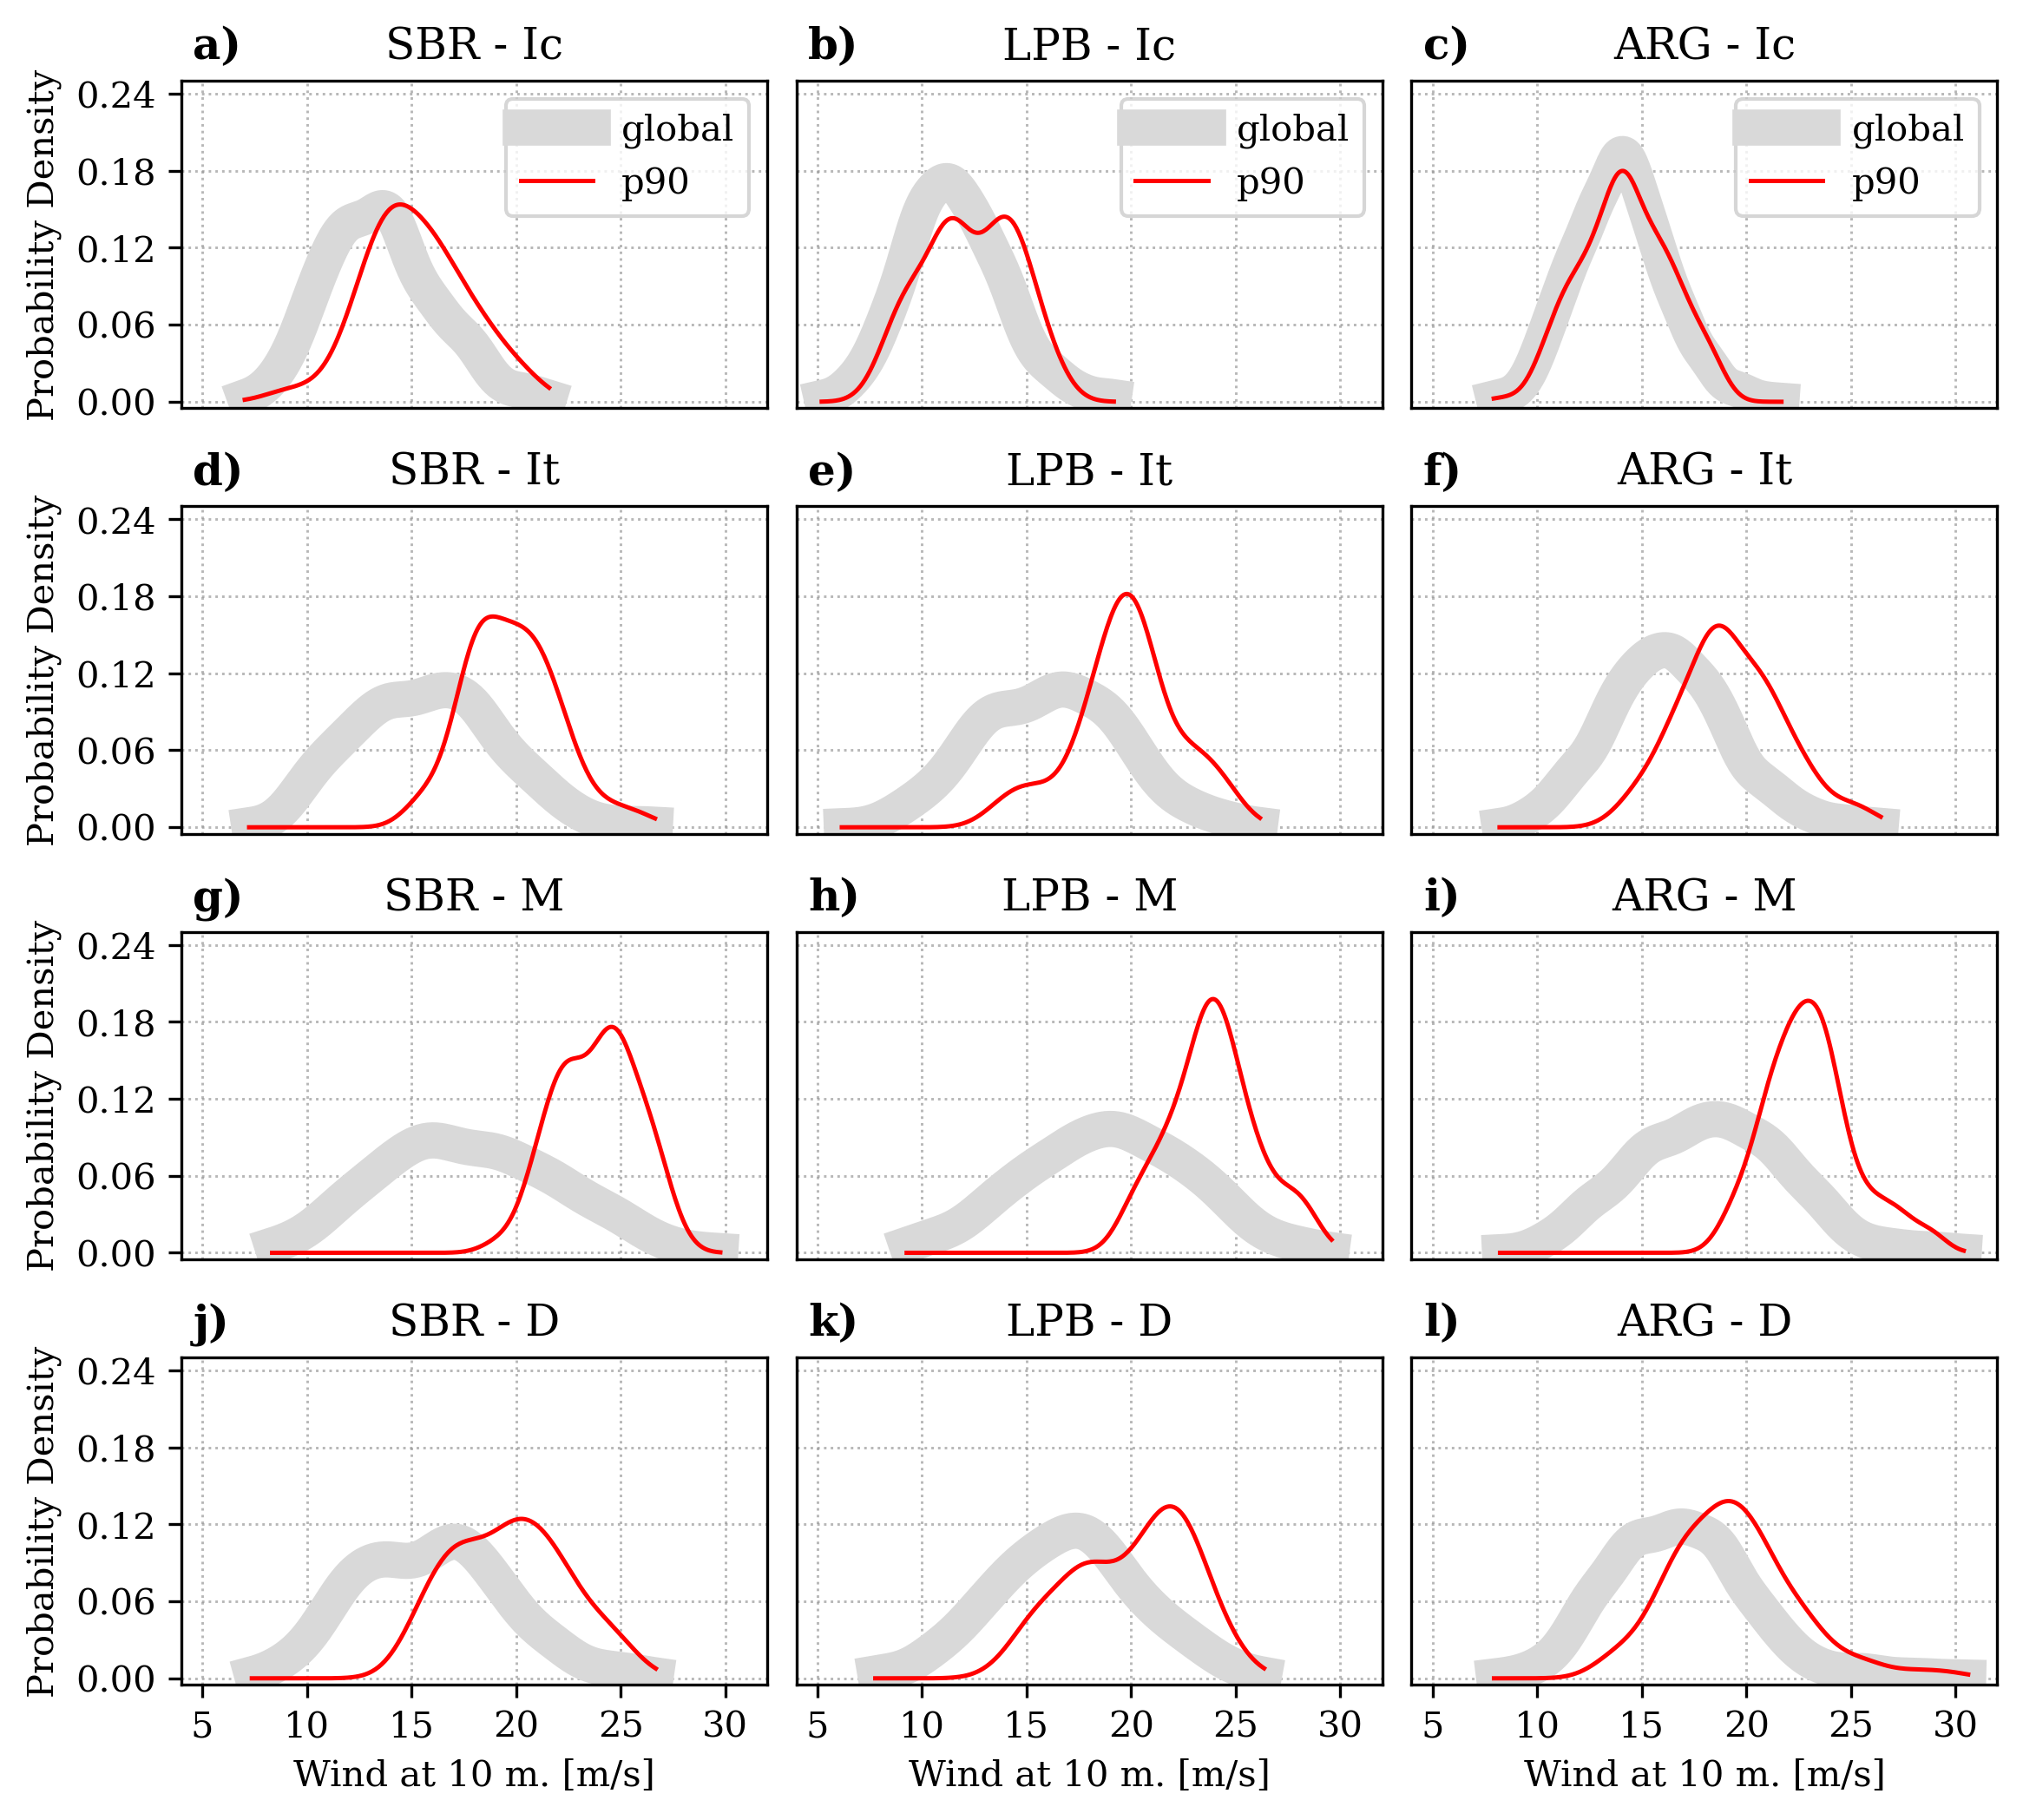
\includegraphics[width=\textwidth]{images/w10/PDF_wind10_sigma025.png}
\caption[PDF de magnitudes máximas de viento a 10 metros]{Funciones de densidad de probabilidad (PDF) para las magnitudes máximas de viento a 10 metros. Las columnas indican la región de ciclogénesis (SBR, LPB, ARG) y las filas la evolución a través de las fases del ciclo de vida (Ic, It, M, D). Se contrasta la Población Global (referencia, sombreado gris) con los subconjuntos definidos por percentiles de los máximos de vorticidad relativa en 850~hPa alcanzados en su ciclo vital: p90 (sistemas intensos, línea roja).}
\label{fig:pdf_wind10}
\end{figure}

La máxima separación de las distribuciones en madurez refleja el momento en que los ciclones p90 expresan su pleno potencial dinámico, alcanzando su mínimo absoluto de vorticidad relativa a 850~hPa, comportamiento coherente entre ambas poblaciones y presentado en la Tabla~\ref{tab:fase_max_intensidad}.
Como sostiene \citet{gramcianinov2019properties}, SBR y LPB alcanzan mayores intensidades de viento superficial por la influencia de procesos termodinámicos en niveles bajos, como la advección cálida y la convergencia de humedad (Secciones~\ref{subsec:tb_sbr} y~\ref{subsec:tb_lpb}). 
\citet{gozzo2013air} respaldan esta dependencia termodinámica al demostrar que los flujos turbulentos de calor sensible y latente océano-atmósfera, junto a una profunda inyección de humedad, son decisivos para desestabilizar el entorno y retroalimentar el sistema. 
\citet{russo2025impacts} sostienen que, si bien la ciclogénesis inicial depende predominantemente de procesos dinámicos de niveles altos, salvo en casos donde los flujos de calor ya son intensos antes de la formación del sistema, la inyección masiva de humedad y flujos de calor latente resulta fundamental durante intensificación y madurez.

En la costa del sur y sureste de Brasil, \citet{rocha2016estudio} muestran que la difluencia en altura, un cavado en niveles medios y la convergencia en bajos niveles favorecen la ciclogénesis regional.
En ARG, la dinámica baroclínica clásica del frente y la perturbación topográfica de los Andes generan respuestas cinemáticas más variables y distribuciones más aplanadas (Sección~\ref{subsec:tb_arg}).
Pese a la menor disponibilidad de humedad, \citet{gramcianinov2024early} muestran que la amplificación de la onda baroclínica de bajo nivel en ARG produce ciclones con presión central más baja que en SBR y LPB, confirmando que la intensidad del viento en esta región depende menos del forzante termodinámico y más de la dinámica frontal.
Según \citet{gan1994influence}, la interacción con la orografía induce distorsiones espaciales en el flujo de niveles bajos y modifica la estructura de las ondas \citep{vera2002cold}.
Este entorno está condicionado por la baroclinicidad ambiental y los gradientes térmicos horizontales \citep{yanase2014parameter}, ligado a la incursión de anomalías de vorticidad potencial en niveles altos durante la ciclogénesis en el este continental \citep{crespo2020potential}.

Al confirmar que los ciclones p90 se separan sistemáticamente de la población a medida que maduran, se valida la clasificación basada en vorticidad (Sección~\ref{sec:poblaciones_estudio}). 
En madurez, el subconjunto p90 desplaza su mayor probabilidad hacia los $\sim$23~m\,s$^{-1}$, un incremento de aproximadamente 50\% respecto a la moda de la Población Global ($\sim$15~m\,s$^{-1}$), con colas que alcanzan hasta 30~m\,s$^{-1}$. 
Este corrimiento es coherente con los rangos reportados para ciclones intensos del Atlántico Sur \citep{padilhareinke2026characterization, gramcianinov2020analysis}.
\citet{padilhareinke2026characterization} documentan para el conjunto del Atlántico Sudoccidental un umbral p90 de 23.4~m\,s$^{-1}$ (84.4~km\,h$^{-1}$) y extremos de hasta 31.4~m\,s$^{-1}$ (113.2~km\,h$^{-1}$).
Este valor resulta del mismo orden de magnitud que el reportado por \citet{gentile2025response} para los ciclones más intensos del Atlántico Norte (${\sim}$25~m\,s$^{-1}$ en vorticidad máxima), pese a tratarse de una población de ciclones y una cuenca oceánica distintas.
\citet{gramcianinov2020analysis} reportan para el invierno austral (JJA) en ERA5 velocidades máximas medias de 21.2\,$\pm$\,4.8~m\,s$^{-1}$ (percentil~90: 27.3~m\,s$^{-1}$; percentil~95: 29.3~m\,s$^{-1}$).\footnote{En el reanálisis CFSR/CFSv2, los valores son ligeramente superiores, 23.4\,$\pm$\,4.8~m\,s$^{-1}$ (percentil~90: 30.2~m\,s$^{-1}$; percentil~95: 32.1~m\,s$^{-1}$) \citep{gramcianinov2020analysis}.} 
Como subraya \citet{gramcianinov2023impact}, identificar tempranamente estos sistemas intensos es indispensable, pues sus vientos anómalos constituyen forzantes de eventos que suponen riesgo directo para regiones costeras y marítimas.

% --- SECCIÓN PRINCIPAL: KDE ESPACIAL DE VIENTO A 10 METROS,

\section{Distribución espacial de máximos (PDFe)}\label{sec:pdfe_wind10}
\subsection{Población Global}\label{sec:kde_espacial_global}

\begin{figure}[htbp]
\centering
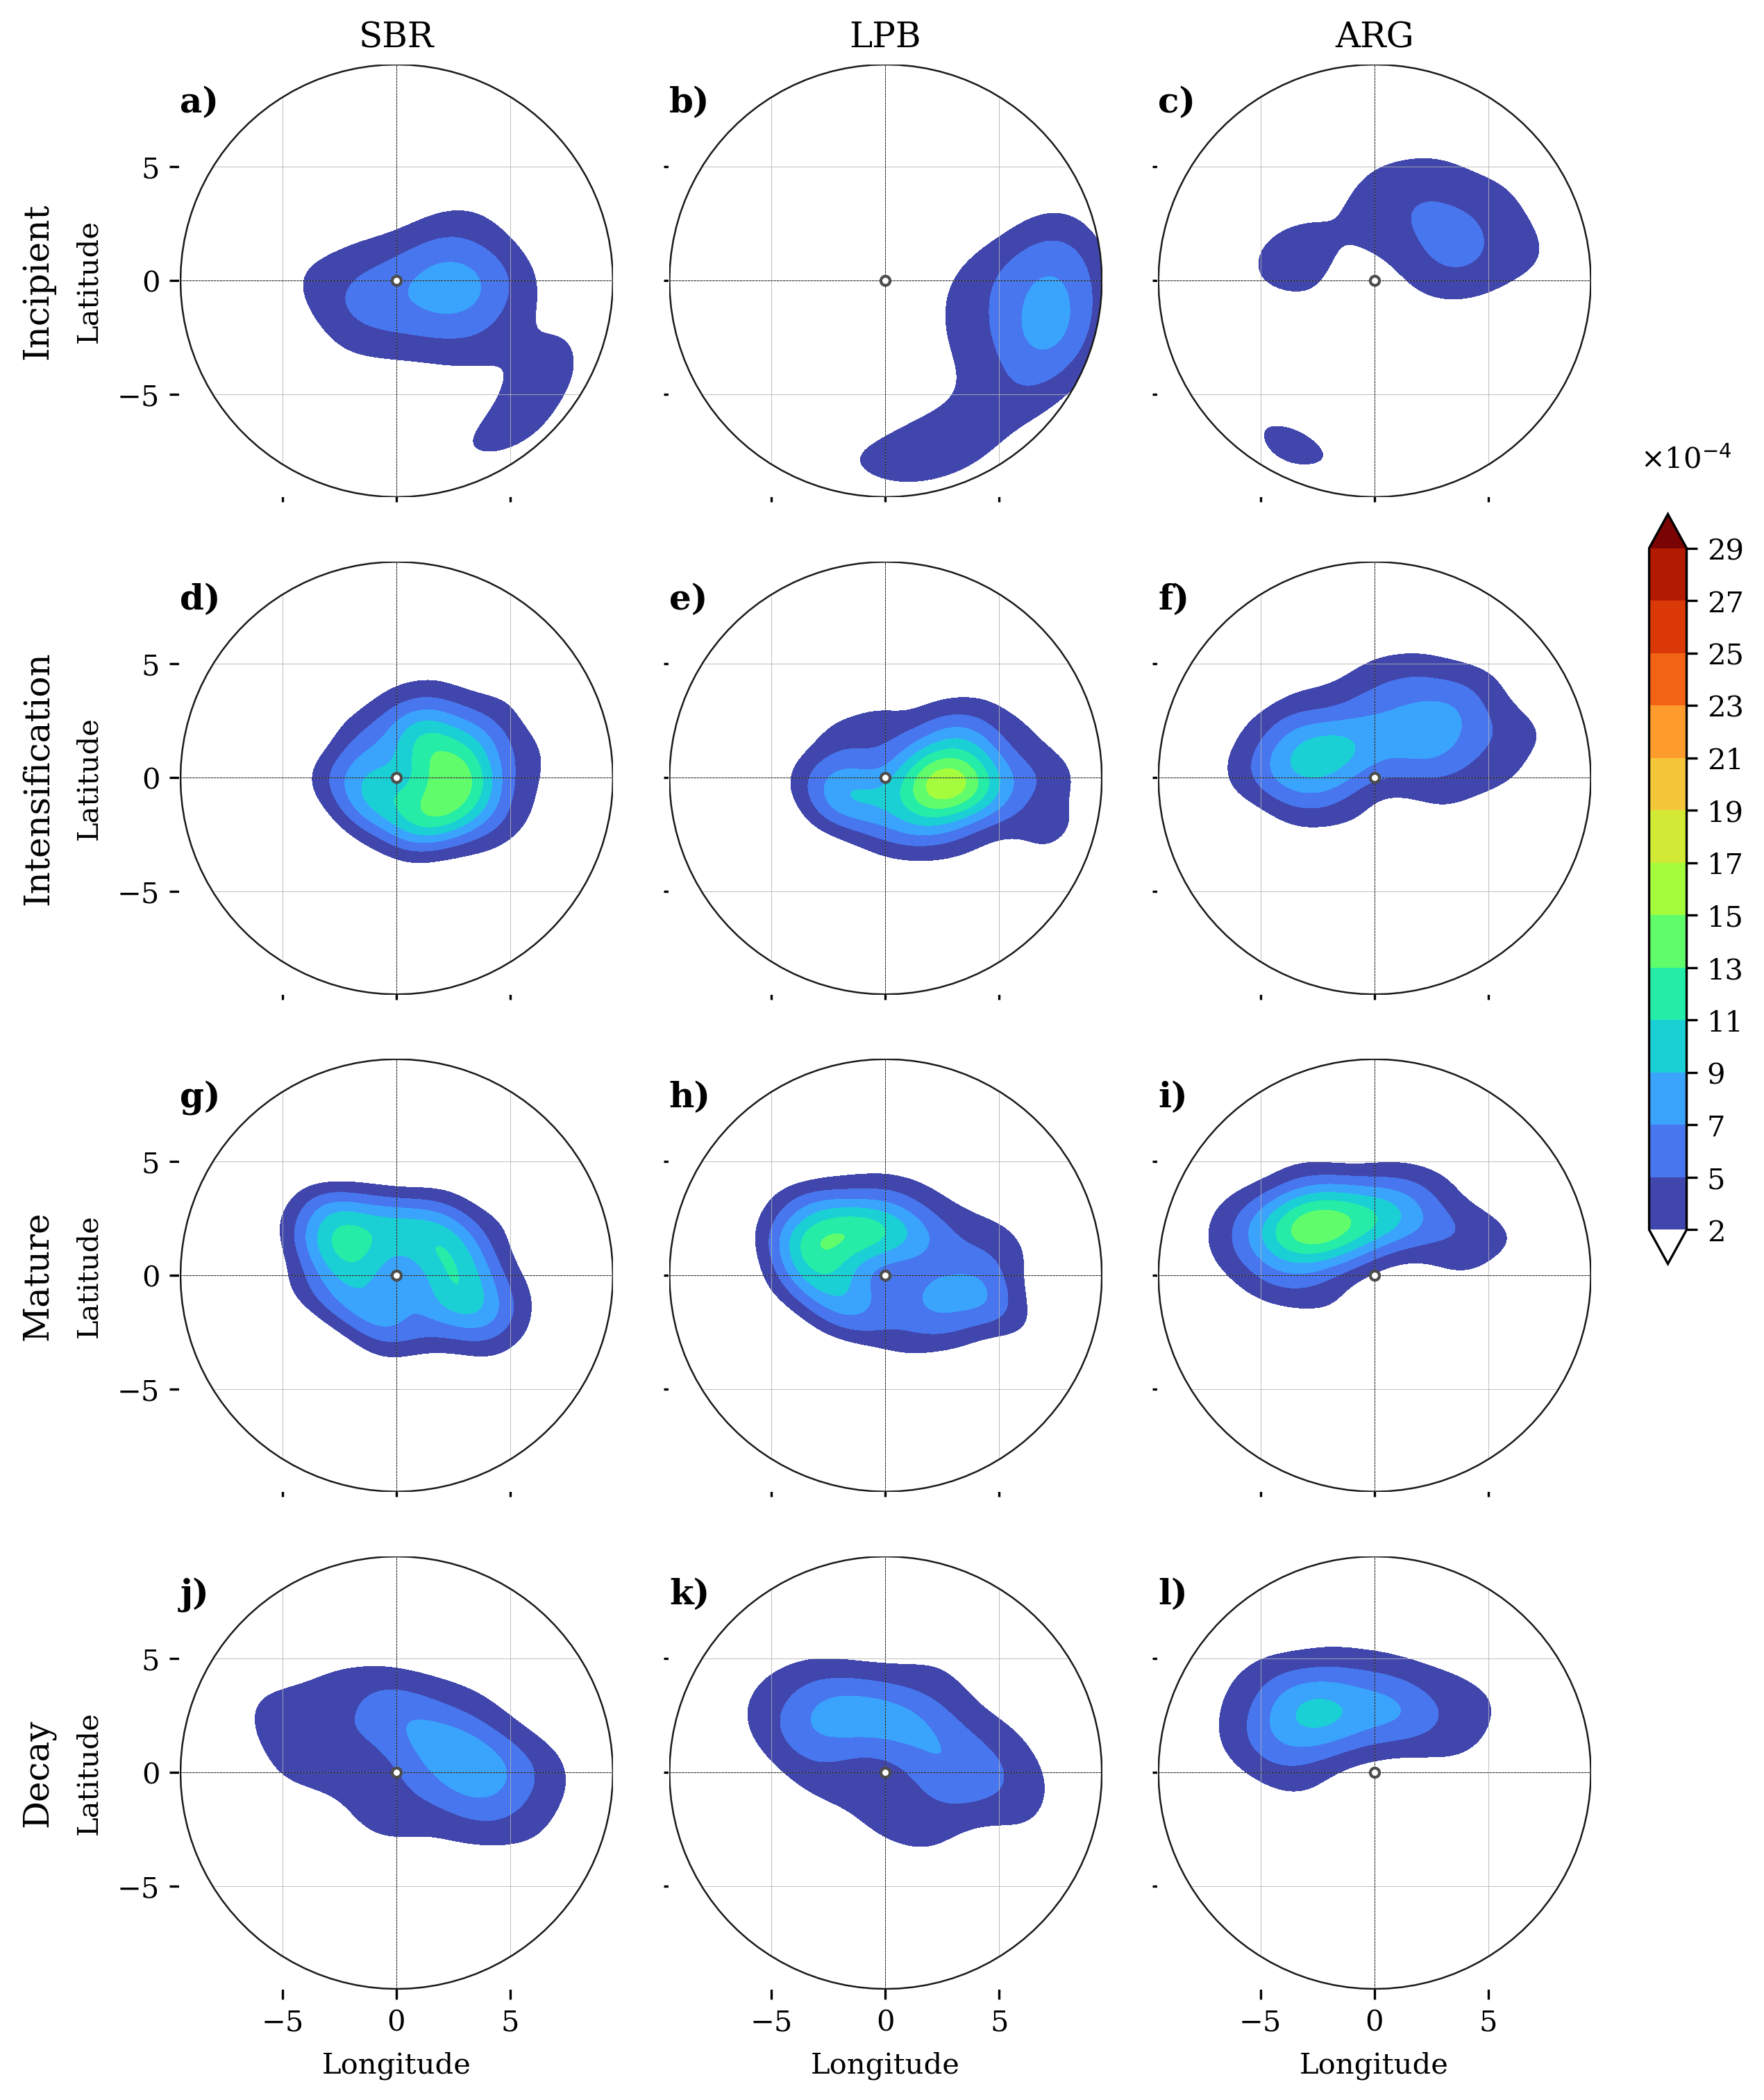
\includegraphics[width=\textwidth]{images/w10/kde_wind10_global_fasesxreg.png}
\caption[PDF espacial de viento máximo a 10 metros --- Población Global]{Estimación de densidad espacial bidimensional (PDFe; Sección~\ref{subsec:kde_localizacion}) de la ubicación de los máximos de magnitud de viento a 10~metros para la Población Global. Las columnas separan las regiones de ciclogénesis (SBR, LPB, ARG) y las filas indican las fases evolutivas (Ic, It, M, D). El dominio lagrangiano está centrado en el ciclón ($0^{\circ}, 0^{\circ}$).}
\label{fig:kde_wind_global}
\end{figure}

La Figura~\ref{fig:kde_wind_global} presenta el campo de densidad espacial sobre el dominio lagrangiano de $20^{\circ} \times 20^{\circ}$ (Sección~\ref{sec:procesamiento_lagrangiano}). 
La distribución es amplia, difusa y con gradientes suaves, sin concentración comparable a la de p90 en ninguna fase o región. 
Esta dispersión es la firma esperada de una población heterogénea, coherente con los métodos de detección basados en vorticidad de \citet{sinclair1994objective}, lo que sugiere un rasgo estructural de la climatología ciclónica y no un efecto metodológico.

La evolución por fases revela una transición espacial. El núcleo de máxima densidad se origina en el sector este durante la incipiencia, se desplaza progresivamente hacia el oeste y se concentra durante la intensificación, y se consolida en el cuadrante noroeste durante la madurez, antes de perder coherencia posicional en el decaimiento.
En las fases iniciales (Ic; paneles a, b y~c), las zonas de máxima densidad abarcan áreas extensas sin estructura simétrica, con el núcleo situado en el sector este (noreste en el caso de ARG), coherente con el comportamiento propio de la fase incipiente, donde los sistemas presentan circulaciones asimétricas antes de organizar un centro de vorticidad cerrado (Sección~\ref{subsec:tb_fases}).
Durante intensificación (It; paneles d, e y~f) las distribuciones transitan hacia estructuras más compactas y cercanas al centro, desplazándose ligeramente hacia el oeste, salvo en ARG, donde el núcleo transita directamente hacia el noroeste, coherente con la consolidación progresiva de la circulación ciclónica en esta fase (Sección~\ref{subsec:tb_fases}).
LPB (e) presenta el núcleo de mayor densidad (${\approx}$\,17--19\,$\times10^{-4}$), sugiriendo una localización más recurrente de los vientos máximos durante esta fase; ARG (f) exhibe una distribución más elongada zonalmente, con mayor dispersión posicional.
Al avanzar hacia madurez (M; paneles g, h e~i) se consolida el desplazamiento del foco de mayor densidad hacia el cuadrante noroeste en las tres regiones, con densidades marcadamente mayores en ARG, con diferencias regionales que se discuten a continuación.
En decaimiento (D; paneles j, k y~l), las densidades caen considerablemente, aproximándose a los valores de la fase incipiente, y la ubicación del núcleo pierde la coherencia posicional que sí caracteriza a la intensificación y la madurez. A diferencia de esas fases, en decaimiento no se observa una concordancia clara de cuadrante entre regiones, comportamiento independiente de la región de ciclogénesis.

El contraste regional más marcado ocurre en madurez. ARG (i) alcanza ${\approx}$\,17--19\,$\times10^{-4}$ concentradas en un único núcleo bien definido, mientras SBR (g) y LPB (h) exhiben valores menores repartidos en dos focos de distinta densidad. 
Como sugiere \citet{yanase2014parameter}, esta evolución espacial asimétrica se liga a zonas baroclínicas donde los máximos gradientes térmicos horizontales interactúan con los chorros en la alta troposfera. 
En ARG el patrón responde a la advección térmica y la perturbación topográfica andina; en SBR y LPB, a la advección de aire cálido y húmedo (Sección~\ref{sec:pdf_wind10}).

La dispersión de la Población Global refleja además la amplia variabilidad en la distancia al centro donde ocurren los vientos máximos. En el Atlántico Sur, \citet{gozzo2014subtropical} y \citet{cardoso2020wind} sitúan estos máximos entre 300-450~km y 400-500~km del centro, respectivamente. Esta heterogeneidad justifica metodológicamente la estratificación por intensidad (Sección~\ref{subsec:subconjuntos_intensidad}). \citet{corner2025classification} y \citet{eisenstein2023identification} señalan que la diversidad estructural exige aislar los eventos severos, práctica habitual en el Hemisferio Norte pero aún insuficientemente sistemática en el Hemisferio Sur. La organización geométrica de los sistemas intensos se examina a continuación, tomando esta población como línea base.

\subsection{Subconjunto de ciclones intensos p90}\label{sec:kde_espacial_p90}

\begin{figure}[htbp]
\centering
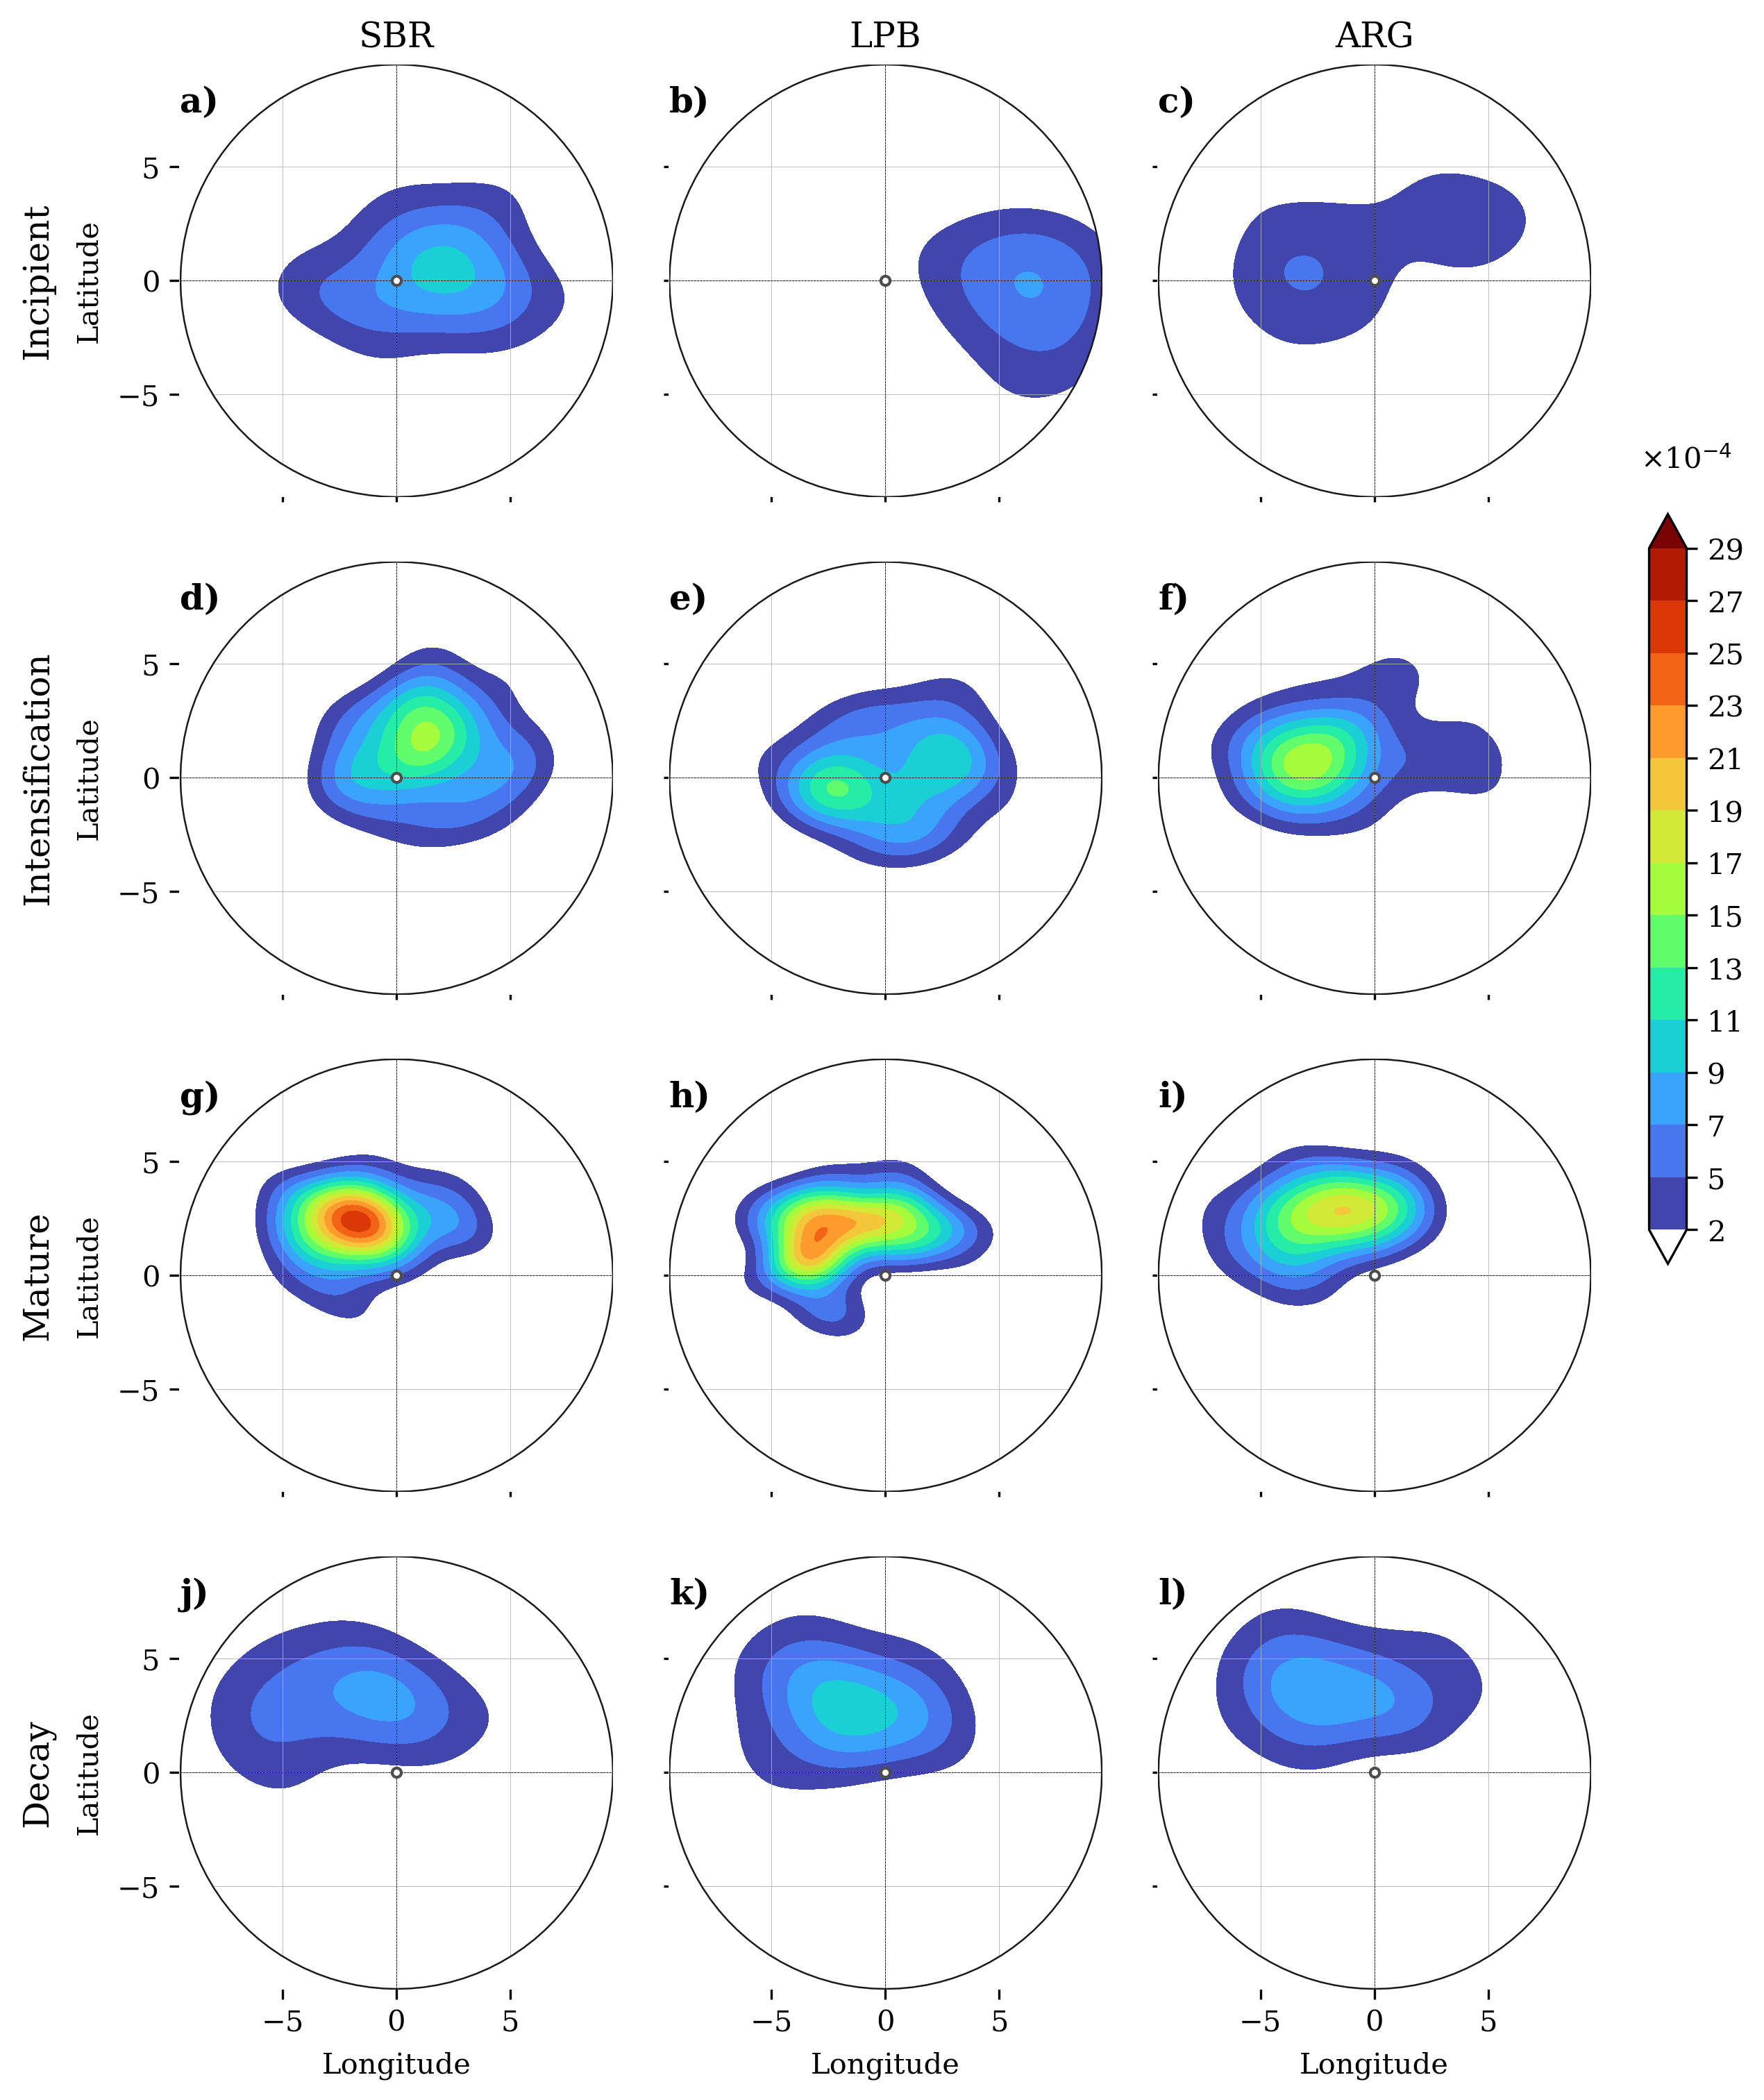
\includegraphics[width=\textwidth]{images/w10/kde_wind10_p90_fasesxreg.png}
\caption[PDF espacial de viento máximo a 10 metros --- Subconjunto p90]{Estimación de densidad espacial bidimensional (PDFe; Sección~\ref{subsec:kde_localizacion}) de la ubicación de los máximos de magnitud de viento a 10~metros para el subconjunto de ciclones intensos. El formato, dominio lagrangiano, fases evolutivas y escala de densidad ($10^{-4}$) son idénticos a los presentados en la Figura~\ref{fig:kde_wind_global} para permitir la comparación estructural directa de las asimetrías de densidad.}
\label{fig:kde_wind_p90}
\end{figure}

Al contrastar la línea base con el subconjunto p90, la reorganización espacial es marcada. La estructura de los vientos máximos deja de ser difusa y se consolida progresivamente en un cuadrante preferencial conforme el sistema evoluciona. La Figura~\ref{fig:kde_wind_p90} documenta esta transición para las cuatro fases y tres regiones.

En fases iniciales (Ic; paneles a, b y~c), las tres regiones mantienen densidad baja y zona de preferencia poco definida, análogo a la Población Global. Al intensificarse (It; paneles d, e y~f), los núcleos inician su desplazamiento hacia el noroeste. En SBR (d) el núcleo se ubica aún al este pero cerca del centro, desplazado hacia la izquierda respecto a la fase incipiente sin alcanzar todavía el cuadrante noroeste; en LPB (e) el núcleo principal ya se sitúa al oeste, ligeramente suroeste, acompañado de un núcleo secundario de menor densidad al este; en ARG (f) el foco aumenta drásticamente respecto a la fase precedente, anticipando la concentración de la madurez.
El cambio más notorio ocurre en madurez (M; paneles g, h e~i). Se configura un núcleo hiperconcentrado en el cuadrante noroeste, entre $-1^{\circ}$ y $-3^{\circ}$ de longitud y $+2^{\circ}$ a $+3^{\circ}$ de latitud relativa al centro.
Las magnitudes en SBR (g) son extremas (23--27\,$\times 10^{-4}$); LPB (h) alcanza ${\approx}$\,23--25\,$\times 10^{-4}$; ARG (i) exhibe una concentración notablemente menor (${\approx}$\,17--19\,$\times 10^{-4}$) y un núcleo menos compacto. Este mismo orden regional (SBR $>$ LPB $>$ ARG) ya aparecía en la magnitud del viento (PDF, Sección~\ref{sec:pdf_wind10}): la región que más concentra la intensidad también concentra más su ubicación.
En decaimiento (D; paneles j, k y~l), el núcleo permanece anclado en el noroeste, a diferencia de la Población Global, donde en SBR y LPB los máximos se dispersaban hacia el norte e incluso el noreste.

Esta hiperconcentración noroeste constituye la firma espacial cinemática de los ciclones profundos maduros del Hemisferio Sur. 
Patrones análogos se documentan en ETC del Hemisferio Norte, donde los vientos extremos se empaquetan en la zona de fractura frontal asociada a chorros de bajo nivel como los \textit{sting jets} y el chorro de la cinta transportadora fría (CCB, \textit{cold conveyor belt}) \citep{clark2005sting, clark2018sting}, cuya proximidad espacio-temporal los vuelve prácticamente indistinguibles en superficie \citep{eisenstein2023identification}; la inversión de la circulación entre hemisferios traslada dicho sector al cuadrante noroeste en el Hemisferio Sur.
Bajo esta misma inversión hemisférica, el máximo de viento superficial que \citet{rudeva2011composite} localizan de forma robusta en el sector suroeste de ciclones del Atlántico Norte predeciría, para el Hemisferio Sur, una concentración en el cuadrante noroeste, coincidente con la hiperconcentración aquí documentada.
Ya el compuesto de \citet{catto2010climate} sobre los 100 ciclones más intensos del Hemisferio Norte en invierno había situado el viento máximo a 925~hPa en ${39.1 \pm 3.5}$~m\,s$^{-1}$, a un radio de ${5.1^{\circ} \pm 2.7^{\circ}}$ del centro y sistemáticamente en el cuadrante trasero-derecho del sistema (la región del WCB), con una metodología de compositing afín a la aquí empleada. \citet{hodges2011comparison} muestran en composites de ciclones intensos que los máximos de viento se localizan a la izquierda de la dirección de propagación, mientras \citet{laurila2021characteristics} confirman que dichas rachas migran hacia el sector posterior, concentrándose tras el frente frío. 
De manera consistente, \citet{priestley2022improved} documentan que los máximos superficiales asociados al CCB se organizan a un radio de ${\sim}$3--3.5$^{\circ}$ del centro ciclónico y en el flanco posterior, geometría coherente con el núcleo aquí identificado. 
Esta recurrencia no se limita al Atlántico Norte. La climatología global más reciente de \citet{gray2024global}, que rastrea precursores de \textit{sting jet} en los tres océanos durante 43 inviernos, muestra que el mecanismo de seclusión cálida y fractura frontal asociado a esta concentración de viento también opera en el Hemisferio Sur, aunque con menor frecuencia relativa (${\sim}$15\% del decil superior de intensidad, frente a ${\sim}$27\% en el Hemisferio Norte).

La consolidación de este núcleo responde a procesos de transferencia de cantidad de movimiento. En las inmediaciones del frente frío se desarrollan intensas corrientes descendentes que transportan momento horizontal de la alta troposfera hacia la capa límite, con una frecuencia hasta 15\% mayor en el sector suroeste del ciclón en climatologías del Hemisferio Norte, que por inversión hemisférica corresponde al noroeste austral aquí documentado \citep{hyeok2024extrem}. Como precisan \citet{martinez2014cold} (Sección~\ref{subsec:tb_modelos}), los vientos más intensos en la retaguardia del núcleo son producto combinado de la CCB, cuyo chorro de bajo nivel se intensifica por el aumento de vorticidad potencial inducido diabáticamente bajo el ascenso de la cinta cálida \citep{schemm2014linkage, blanchard2021warm}.

Además, \citet{gentile2023observed} muestran que el CCB en ciclones maduros ocurre en capas límite más profundas e inestables en el sector frío, favoreciendo la mezcla descendente de aire de alta velocidad hacia la superficie, lo que se manifiesta en la PDFe como empaquetamiento localizado. Aunque \citet{stankovic2025surface} reportan extremos absolutos mayores en el Hemisferio Norte por su mayor baroclinicidad, los valores en la cola p90 de la región alcanzan magnitudes similares.

Las diferencias interregionales de la Figura~\ref{fig:kde_wind_p90} --mayor concentración en SBR y LPB respecto a ARG-- respaldan el mismo marco dinámico ya descrito: predominio termodinámico (flujos de calor y humedad) en SBR/LPB frente a control baroclínico-orográfico en ARG (Sección~\ref{sec:pdf_wind10}).

Debe considerarse que los datos de reanálisis ERA5 pueden subestimar la intensidad real del viento por limitaciones de resolución. La incapacidad de resolver explícitamente estructuras de mesoescala conduce a subestimación inherente de las magnitudes extremas \citep{hodges2011comparison, priestley2022improved} (Sección~\ref{sec:tb_compound_def}), lo cual debe considerarse al interpretar los valores absolutos de densidad presentados.

Una referencia observacional directa de la magnitud que puede alcanzar el viento en estas estructuras proviene del caso clásico documentado por \citet{shapiro1990life}. Durante la fase de seclusión cálida de un ETC profundo (presión central ${\sim}935$~hPa) del Atlántico Norte, mediciones de aeronave registraron velocidades de hasta 35--50~m\,s$^{-1}$ en niveles bajos. Aunque no corresponden a viento en superficie a 10~m, la fricción reduce sistemáticamente el viento hacia niveles más bajos, por lo que estos valores son consistentes con las colas de hasta 30~m\,s$^{-1}$ observadas en el wind10 de ERA5 para el subconjunto p90 (Sección~\ref{sec:pdf_wind10}), respaldando que la subestimación de ERA5 es plausible incluso en el extremo superior de la distribución.

\citet{gray2020prototype}, en una herramienta de pronóstico en tiempo real para el Met Office, documenta un caso casi en superficie: durante la tormenta Brendan (Reino Unido, enero de 2020; profundización de 49~hPa en 24~h), el dispersómetro ASCAT registró vientos equivalentes a 10~m superiores a 55~nudos (${\sim}28$~m\,s$^{-1}$) al sur del centro, coincidiendo con el sector señalado como precursor de \textit{sting jet}. Esto ilustra la relevancia práctica --más allá de la académica-- de caracterizar con precisión estos máximos, motivación central de este capítulo.

En conjunto, estos resultados demuestran que el grado de intensidad de un ciclón predetermina su patrón espacial. Los sistemas intensos del Atlántico Sur concentrarán casi invariablemente sus máximos de viento a 10~metros en un radio y cuadrante particular respecto a su centro. Esta previsibilidad geométrica resulta necesaria para modelar la distribución espacial exacta del acoplamiento cinemático entre el ciclón y la capa límite superficial.
%%%%%%%%%%%%%
% --- SECCIÓN: PATRONES DOMINANTES DE VARIABILIDAD (EOF) - VIENTO A 10 METROS,
\section{Organización estructural: Análisis EOF}\label{sec:eof_wind10}
\subsection{Fraccionamiento de varianza}\label{sec:var_exp_wind10}
\begin{figure}[htbp]
\centering
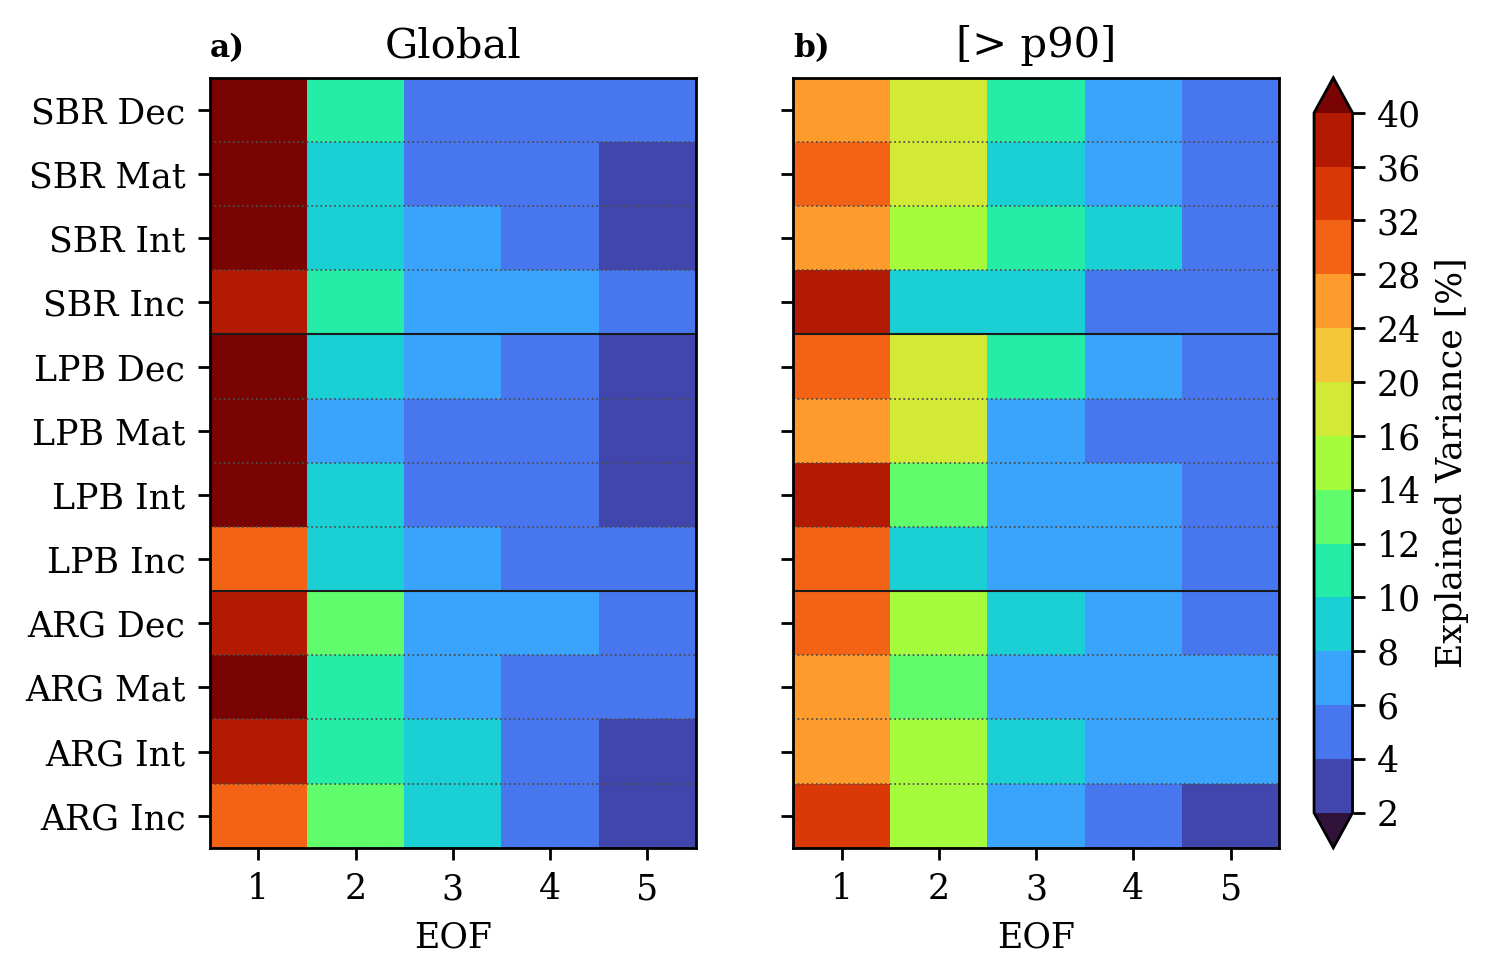
\includegraphics[width=0.8\textwidth]{images/w10/all_expvar_wind10_mean2times.png}
\caption[Varianza explicada por los primeros cinco modos (EOF1--EOF5) de viento a 10~m]{Fraccionamiento de la varianza espacial total contenida en los primeros cinco modos dominantes (EOF1 a EOF5) del viento a 10~metros, obtenida mediante el procedimiento descrito en la Sección~\ref{subsec:eof_univariado}. Se contrasta la distribución de la varianza de la Población Global frente al subconjunto de intensidad p90 a lo largo del ciclo de vida para cada región de ciclogénesis.}
\label{fig:var_exp_wind10}
\end{figure}

La Figura~\ref{fig:var_exp_wind10} resume la varianza distribuida en los primeros cinco modos ortogonales (EOF1 a EOF5), contrastando la Población Global (panel~a) frente al subconjunto p90 (panel~b). En la Población Global, EOF1 domina sobre los modos secundarios en todas las regiones y fases, con concentración máxima en madurez: 57.4\% en SBR y 57.1\% en LPB, con caída abrupta hacia los modos secundarios. ARG presenta valores algo menores, entre 30.9\% y 43.3\%. Este patrón refuerza que la dinámica del viento superficial está gobernada por un único patrón espacial dominante en la Población Global, compatible con un gradiente de gran escala, como el flujo sinóptico de fondo (Sección~\ref{subsec:eof_univariado}).

En el subconjunto p90, la distribución cambia. EOF1 no supera el 37.6\% en ninguna combinación de región y fase, con mínimos de hasta 25.4\% durante intensificación en ARG. La varianza se reparte entre múltiples modos, elevando la importancia de EOF2 y EOF3. Este aplanamiento del espectro de autovalores es, según \citet{hannachi2007empirical}, indicador de que la energía del sistema se distribuye entre modos competitivos de distinta escala espacial. Esta divergencia responde a la complejidad estructural de los ciclones p90. Al intensificarse, el vórtice adquiere no linealidad, repercutiendo en el frente, corrientes en chorro de bajos niveles y seclusiones térmicas (Sección~\ref{subsec:tb_modelos}). Estructuras de mesoescala competirían por la energía cinética del campo, lo que explicaría que la descomposición requiera múltiples dimensiones ortogonales (EOF2--EOF5) para reconstruir la varianza del campo.

Estos resultados demuestran cuantitativamente que la severidad ciclónica no equivale a un escalado lineal de un sistema ordinario. La necesidad de múltiples modos para explicar los sistemas p90 implica que parametrizar vientos intensos asumiendo los patrones simples de la población media subestimará sistemáticamente tanto la agresividad como la naturaleza asimétrica y la localización de los máximos de viento.
%%%%%%%
\subsection{EOF1 --- Población Global}\label{subsec:eof1_wind10_global}

\begin{figure}[htbp]
\centering
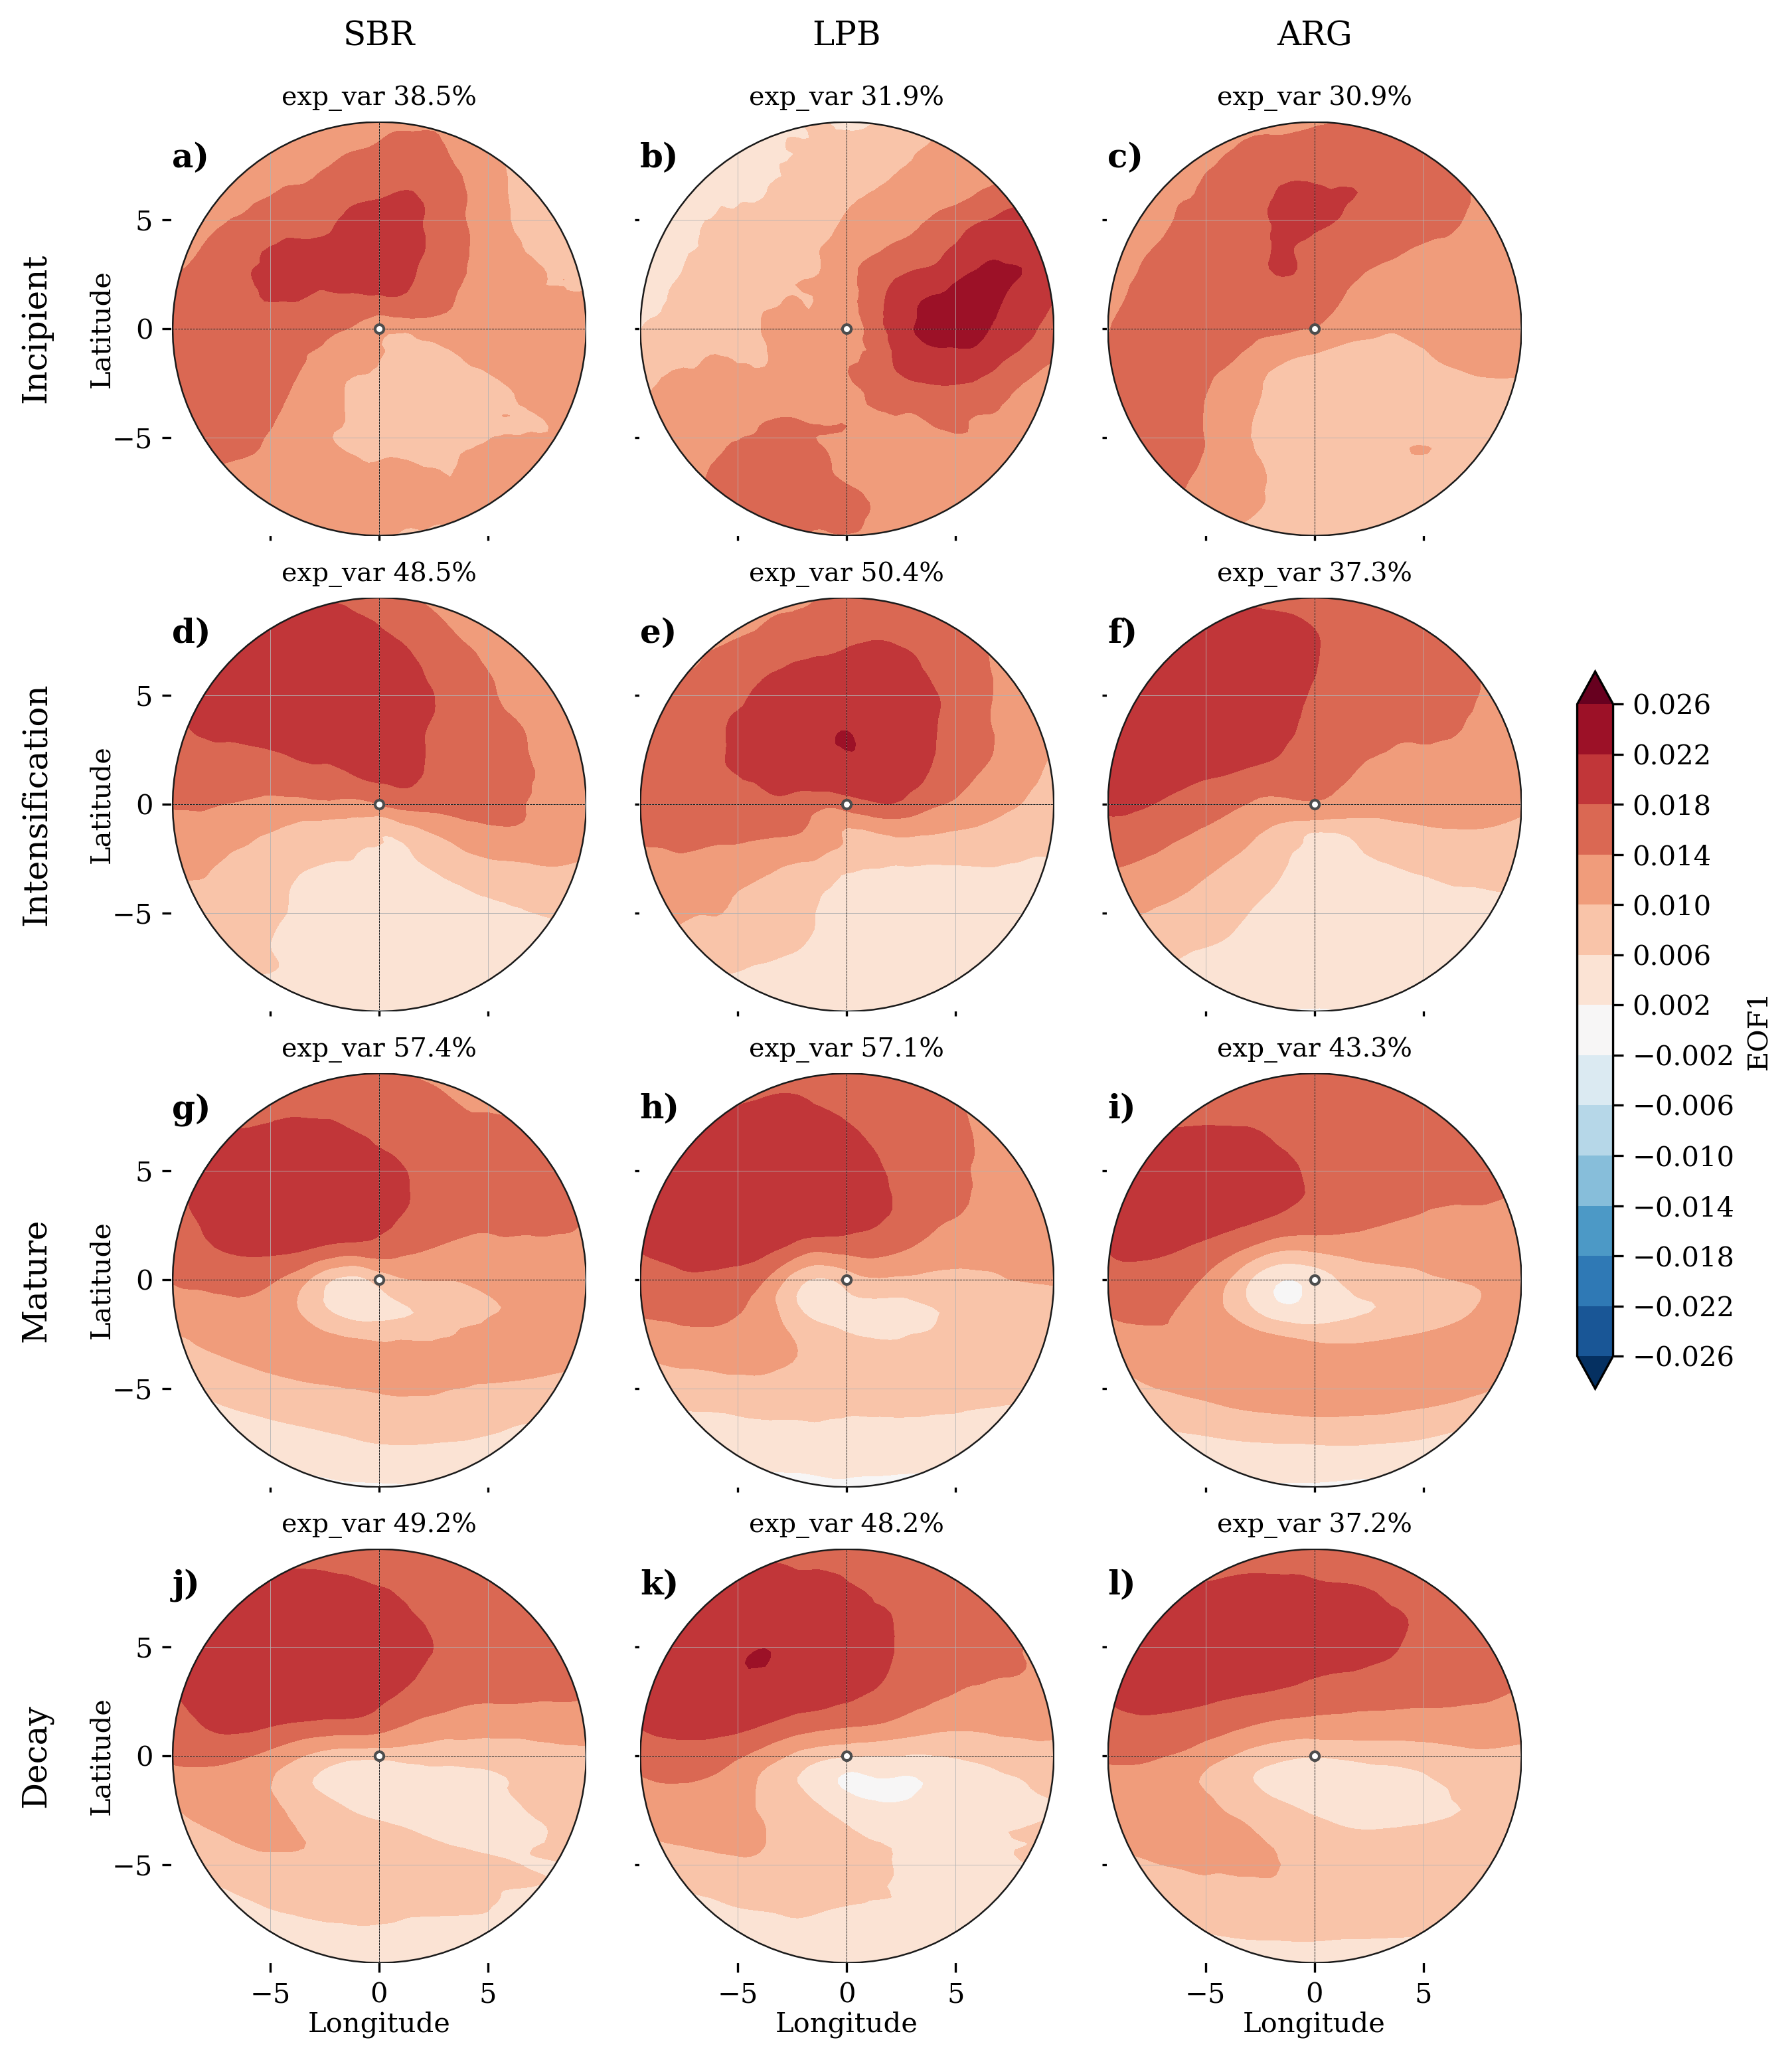
\includegraphics[width=\textwidth]{images/w10/pca1_wind10_global_fasesxreg.png}
\caption[EOF1 de la magnitud del viento a 10 metros --- Población Global]{Primer modo espacial (EOF1) de la magnitud del viento a 10~metros para la Población Global de referencia, derivado del análisis descrito en la Sección~\ref{subsec:eof_univariado}. Los paneles (a--c) corresponden a la fase incipiente (Ic) para las regiones SBR, LPB y ARG, respectivamente; (d--f) a la intensificación (It); (g--i) a la madurez (M); y (j--l) al decaimiento (D). El título de cada panel indica el porcentaje de varianza explicada (\textit{exp\_var}) por este modo dominante. Los colores cálidos (fríos) representan anomalías positivas (negativas) de la estructura del viento relativo al centro del ciclón en un dominio de $20^{\circ} \times 20^{\circ}$.}
\label{fig:eof1_wind10_global}
\end{figure}

La Figura~\ref{fig:eof1_wind10_global} presenta el EOF1 del campo de viento a 10~metros sobre el dominio lagrangiano. Como se evidencia en el fraccionamiento de energía (Sección~\ref{sec:var_exp_wind10}), EOF1 domina ampliamente la varianza en la Población Global, entre 30.9\% (ARG incipiente) y 57.4\% (SBR madurez) según región y fase. Morfológicamente, el patrón es un débil dipolo norte--sur de gran escala. Las anomalías positivas dominan el sector norte (tonos rojos, $+0.010$ a $+0.026$), mientras que valores próximos a cero se concentran en el sur y en las inmediaciones del centro ciclónico (tonos blancos--rosados tenues). Este dipolo se consolida progresivamente desde la fase incipiente hasta la madurez, donde alcanza su mayor definición espacial y varianza explicada en SBR (g, 57.4\%) y LPB (h, 57.1\%). La excepción es LPB en intensificación (e), donde el núcleo positivo se centraliza próximo al vórtice en lugar de desplazarse hacia el norte-noroeste, patrón morfológicamente distinto al resto. En el decaimiento (j, k, l), las tres regiones se asemejan en la distribución de la huella positiva al noroeste con atenuamiento progresivo hacia el sureste; el dominio adopta una cobertura casi uniforme de anomalías positivas débiles.

La presencia de este patrón norte--sur desde intensificación hasta madurez, junto con su elevada varianza explicada, sugiere que la variabilidad en los ciclones responde, al menos en parte, a su interacción con el flujo zonal de fondo y las fluctuaciones del gradiente latitudinal de temperatura.
Según \citet{hoskins2005new}, hasta el 75\% de los eventos de ciclogénesis en superficie en Sudamérica ya presentan una contraparte ciclónica contemporánea a 500 hPa. Este acoplamiento baroclínico ofrece un marco plausible para el fortalecimiento progresivo del dipolo de EOF1 hasta la madurez, cuando el sistema expandiría su campo de viento en superficie en sintonía con la posición del chorro en altura, expansión que \citet{simmonds2000size} documentan como un aumento sistemático del radio ciclónico durante el desarrollo. La excepción geométrica de LPB en intensificación (e) respalda la dependencia de los forzantes físicos locales. Según \citet{gramcianinov2019properties}, los sistemas en esta zona están modulados en sus etapas iniciales por la influencia de la baja orográfica, lo que ancla la varianza del viento a forzantes topográficos centralizados y retrasa la imposición del débil dipolo zonal de gran escala característico de las demás regiones y fases.

En el decaimiento, al debilitarse el sistema, la circulación ciclónica pierde definición y la variabilidad de su componente cinemática queda supeditada a los desplazamientos del flujo zonal del entorno. La perturbación queda inmersa en el flujo de mayor escala, lo que concuerda con la zonificación que \citet{inatsu2004zonal} describen, quienes documentan que las trayectorias invernales del Hemisferio Sur presentan una asimetría zonal organizada por ondas estacionarias troposféricas, modulando la disipación de los sistemas sinópticos. 
Este patrón univariado establece la línea base de variabilidad estructural de los ETC, necesaria para la comparación con los eventos intensos y con el análisis multivariado (Sección~\ref{sec:meof_prototipos}).
%%%%%%
\subsection{EOF1 --- Subconjunto p90}\label{subsec:eof1_wind10_p90}

\begin{figure}[htbp]
\centering
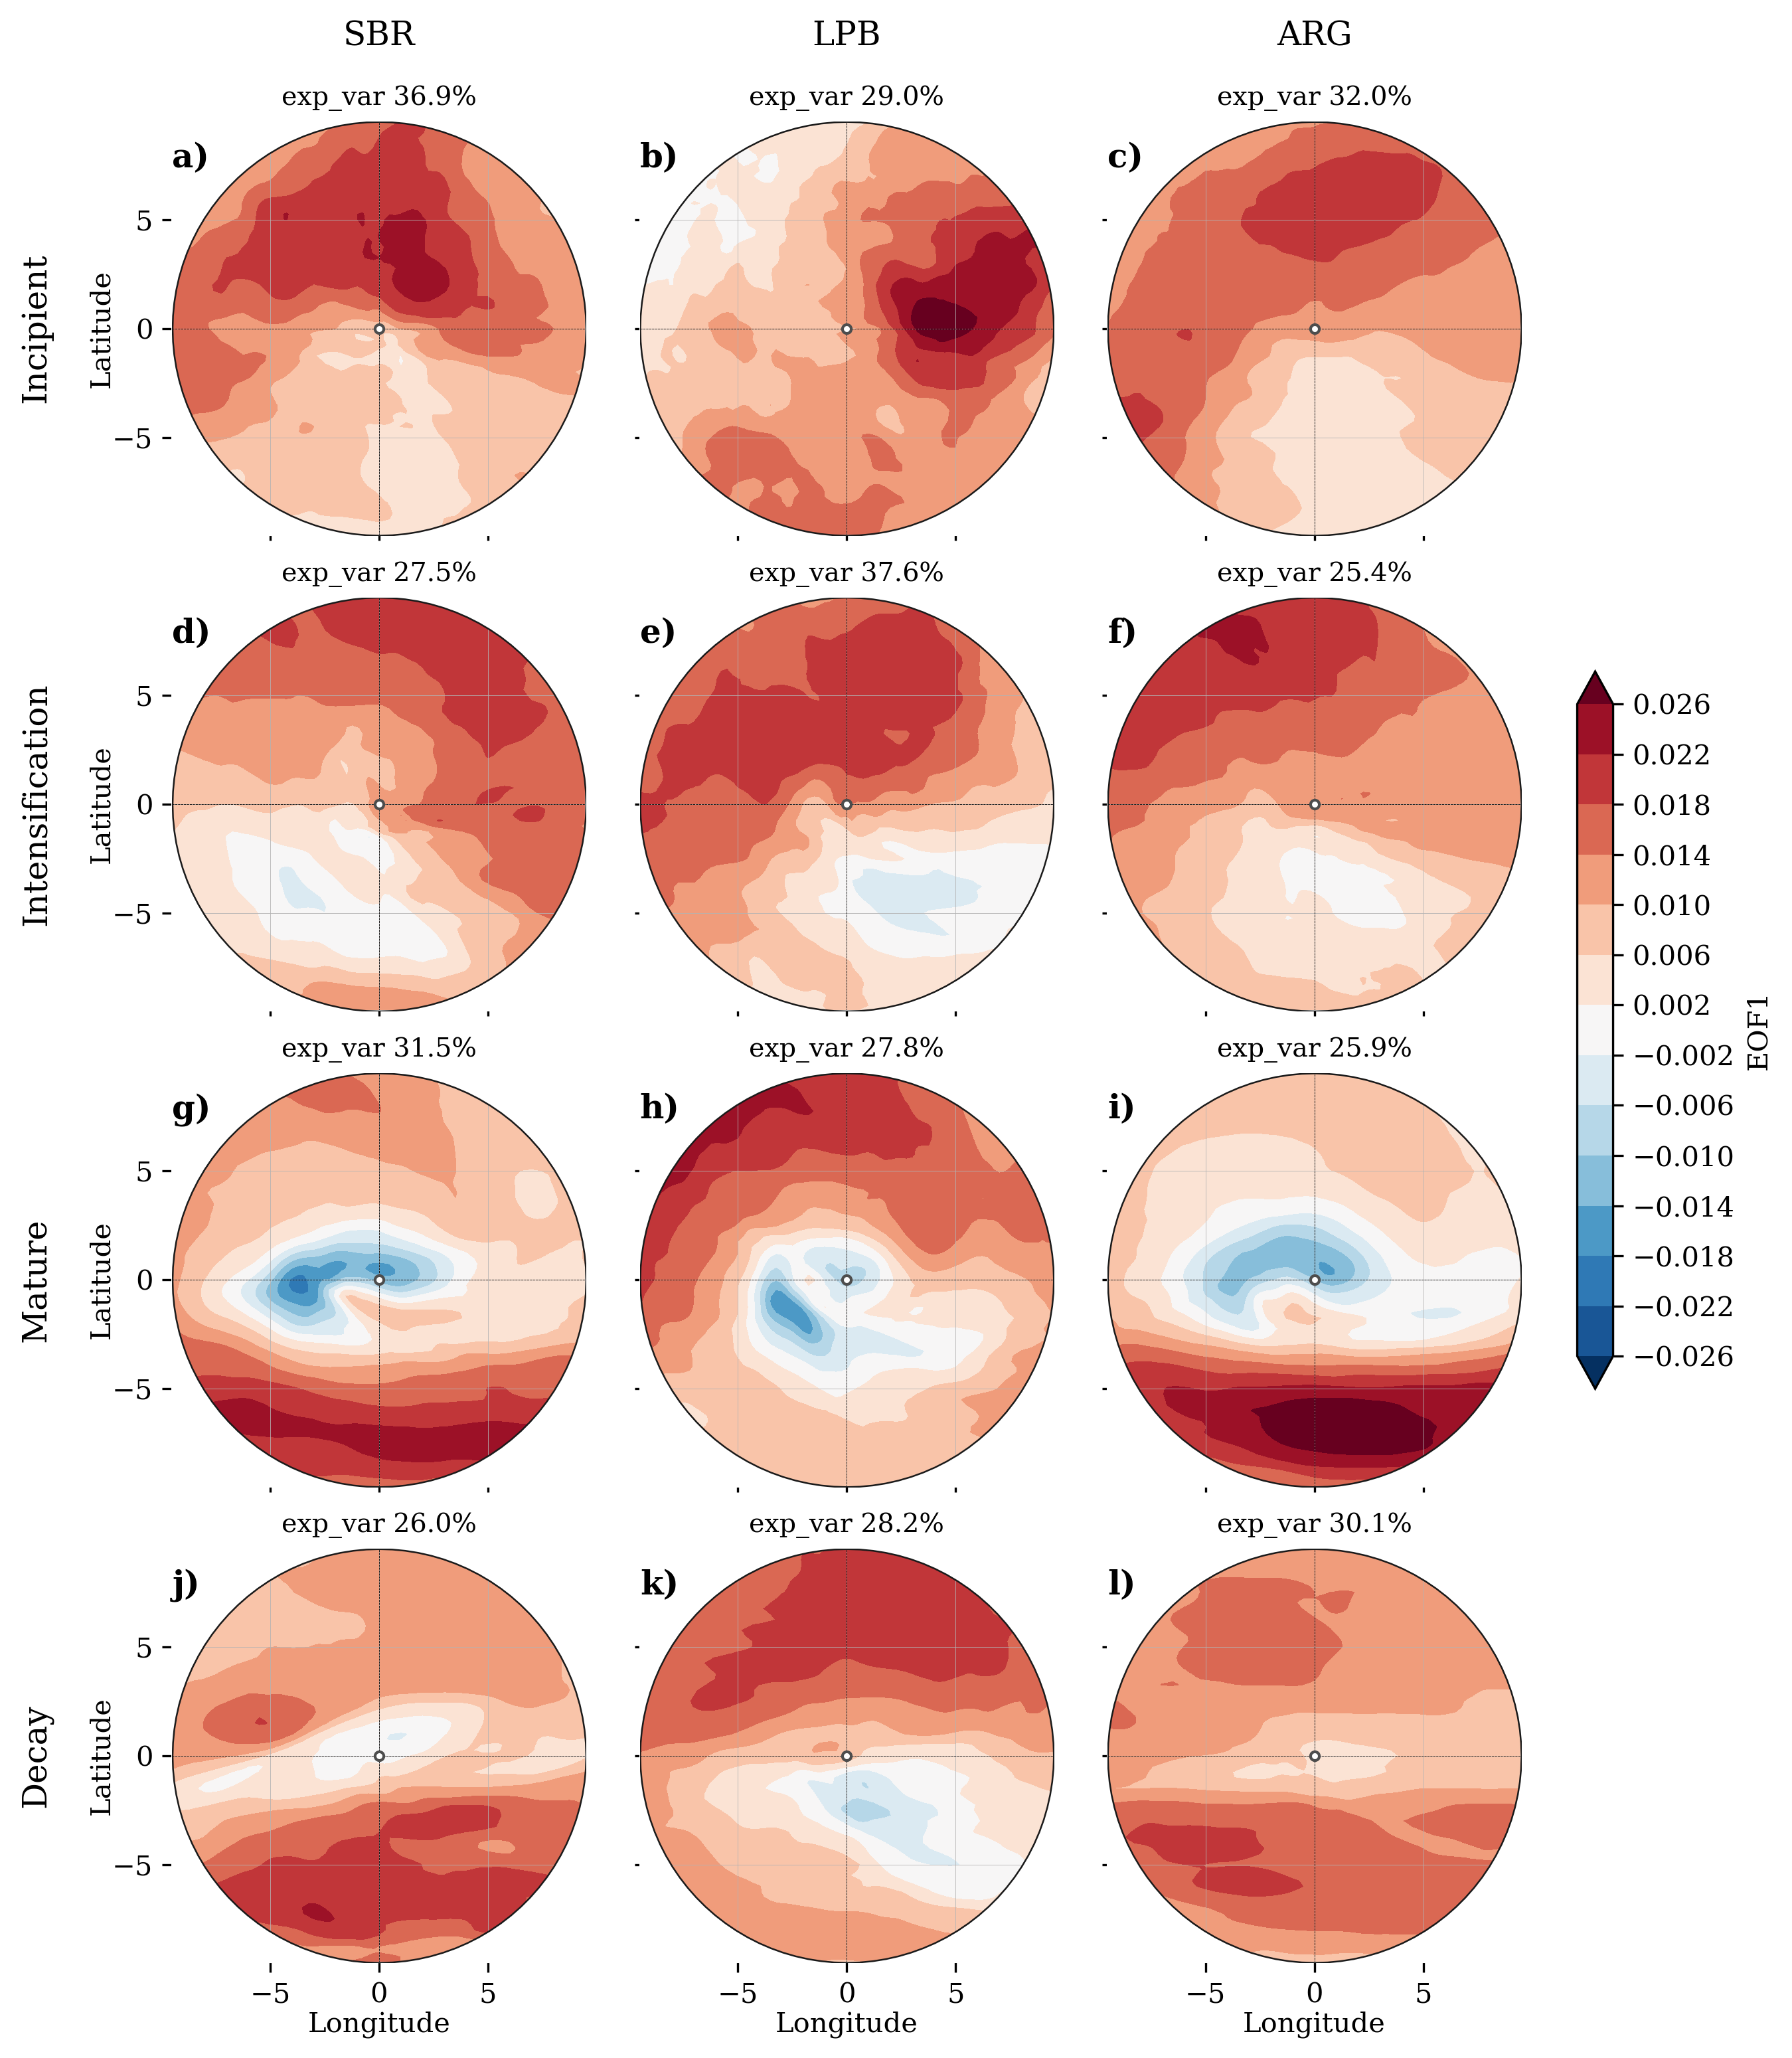
\includegraphics[width=\textwidth]{images/w10/pca1_wind10_p90_fasesxreg.png}
\caption[EOF1 de la magnitud del viento a 10 metros --- Subconjunto p90]{Primer modo espacial (EOF1) de la magnitud del viento a 10~metros para el subconjunto de ciclones intensos (p90). La disposición de los paneles (a--l) por región de ciclogénesis (columnas) y fase evolutiva (filas) es idéntica a la
Figura~\ref{fig:eof1_wind10_global}. Se detalla la varianza explicada (\textit{exp\_var}) en cada panel y la barra de color estandarizada para evaluar
las diferencias en las firmas espaciales de los eventos intensos frente al comportamiento climatológico.}
\label{fig:eof1_wind10_p90}
\end{figure}

El contraste con la Población Global revela que los ciclones p90 no amplifican el patrón base, sino que reconfiguran su estructura modal. En p90, la varianza de EOF1 se reduce, oscilando entre 25.4\% y 37.6\%, y el patrón muestra firmas más complejas e hiperlocalizadas que el débil dipolo norte--sur de gran escala de la Sección~\ref{subsec:eof1_wind10_global}.

La evolución morfológica por fases evidencia esta reconfiguración. En incipiente (a, b, c), las tres regiones muestran patrones difusos con anomalías positivas dominando el norte y noreste, sin estructura dipolar bien definida, coherente con la baja organización esperada. En intensificación (d, e, f) emerge un dipolo norte--sur más definido, con anomalías positivas en norte, noreste y noroeste, y negativas débiles en el sur, con ARG (f) mostrando la señal más intensa ($>+0.022$ en el noroeste). El mayor cambio ocurre en madurez (g, h, i). Las tres regiones desarrollan un dipolo asimétrico con núcleo negativo compacto e intenso al oeste del centro ciclónico, rodeado de anomalías positivas en norte y sur. Este núcleo negativo es particularmente intenso en LPB (h); en SBR (g) y ARG (i) las anomalías negativas son más tenues, extendiéndose en SBR hacia el suroeste con valores de hasta $-0.022$. En decaimiento (j, k, l), el dipolo pierde definición y el dominio retorna a cobertura predominantemente positiva con gradientes más suaves, aunque los contornos negativos se aproximan al núcleo en SBR y LPB.

La hiperlocalización de las anomalías en madurez es la manifestación espacial de la fragmentación de energía multiescalar discutida en la Sección~\ref{sec:var_exp_wind10}. En estos eventos, una circulación cerrada de mesoescala parece ganar peso frente al flujo de fondo: EOF1 deja de tener la forma de un gradiente sinóptico extendido y pasa a describir variabilidad concentrada cerca del núcleo, en posición e intensidad. Esa localización recuerda a la zona donde la literatura sitúa la cinta transportadora fría (CCB) y la fractura frontal (Sección~\ref{sec:kde_espacial_p90}), aunque con el viento escalar aquí disponible no es posible distinguirla de otros mecanismos de escala similar, como el sting jet o la intrusión seca.

El patrón de ARG en madurez (i) merece una lectura diferenciada. La combinación de anomalías negativas intensas en el centro-norte y positivas en el sur configura una firma que indica fluctuaciones en el tamaño de la seclusión cálida (\textit{warm seclusion}; Secciones~\ref{subsec:tb_modelos} y~\ref{subsec:tb_fases}). Como detalla \citet{reboita2022from} para el Atlántico Sur, la formación de esta seclusión en el núcleo es el rasgo evolutivo del modelo conceptual de \citet{shapiro1990life}, vía de desarrollo característica de ciclones con alta organización baroclínica, rodeada por un anillo de vientos según documentan \citet{schultz2021antecedents} y \citet{shapiro1999bridge}.

En conjunto, un ciclón intenso no es estructuralmente equivalente a un ciclón ordinario. Su dinámica modifica la morfología modal del campo de viento. Esta separación concuerda con el espacio de fases de \citet{hart2003cyclone}, que demuestra que las fluctuaciones en la asimetría térmica y el espesor de capa definen caminos evolutivos distintivos. Como enfatizan \citet{corner2025classification} y \citet{eisenstein2023identification}, la intensidad del viento superficial no depende únicamente de la sinóptica de gran escala, sino de la manifestación explícita de estas estructuras mesoescalares internas.
%%%%%%%%
\subsection{Significancia estadística}\label{subsec:res_significancia_madurez}

Para discriminar entre señales físicas y fluctuaciones estocásticas del remuestreo, se evalúa la significancia estadística de los autovectores espaciales mediante el método Bootstrap-t (Sección~\ref{subsec:bootstrap_significancia}), siguiendo a \citet{hesterberg2015bootstrap}. Este análisis se concentra en la fase de madurez, el momento de mayor señal dinámica y de mayor interés para el argumento central de esta tesis, como verificación representativa de que los patrones EOF documentados en las demás fases no son artefactos del muestreo. La Figura~\ref{fig:xeof_madurez_global} documenta los tres primeros modos (EOF1--EOF3) y sus series temporales (PC1--PC3) para la Población Global en madurez, y la Figura~\ref{fig:xeof_madurez_p90} presenta el análisis equivalente para p90. El achurado delimita las áreas estadísticamente significativas al 95\% de confianza.

\begin{figure}[htbp]
\centering
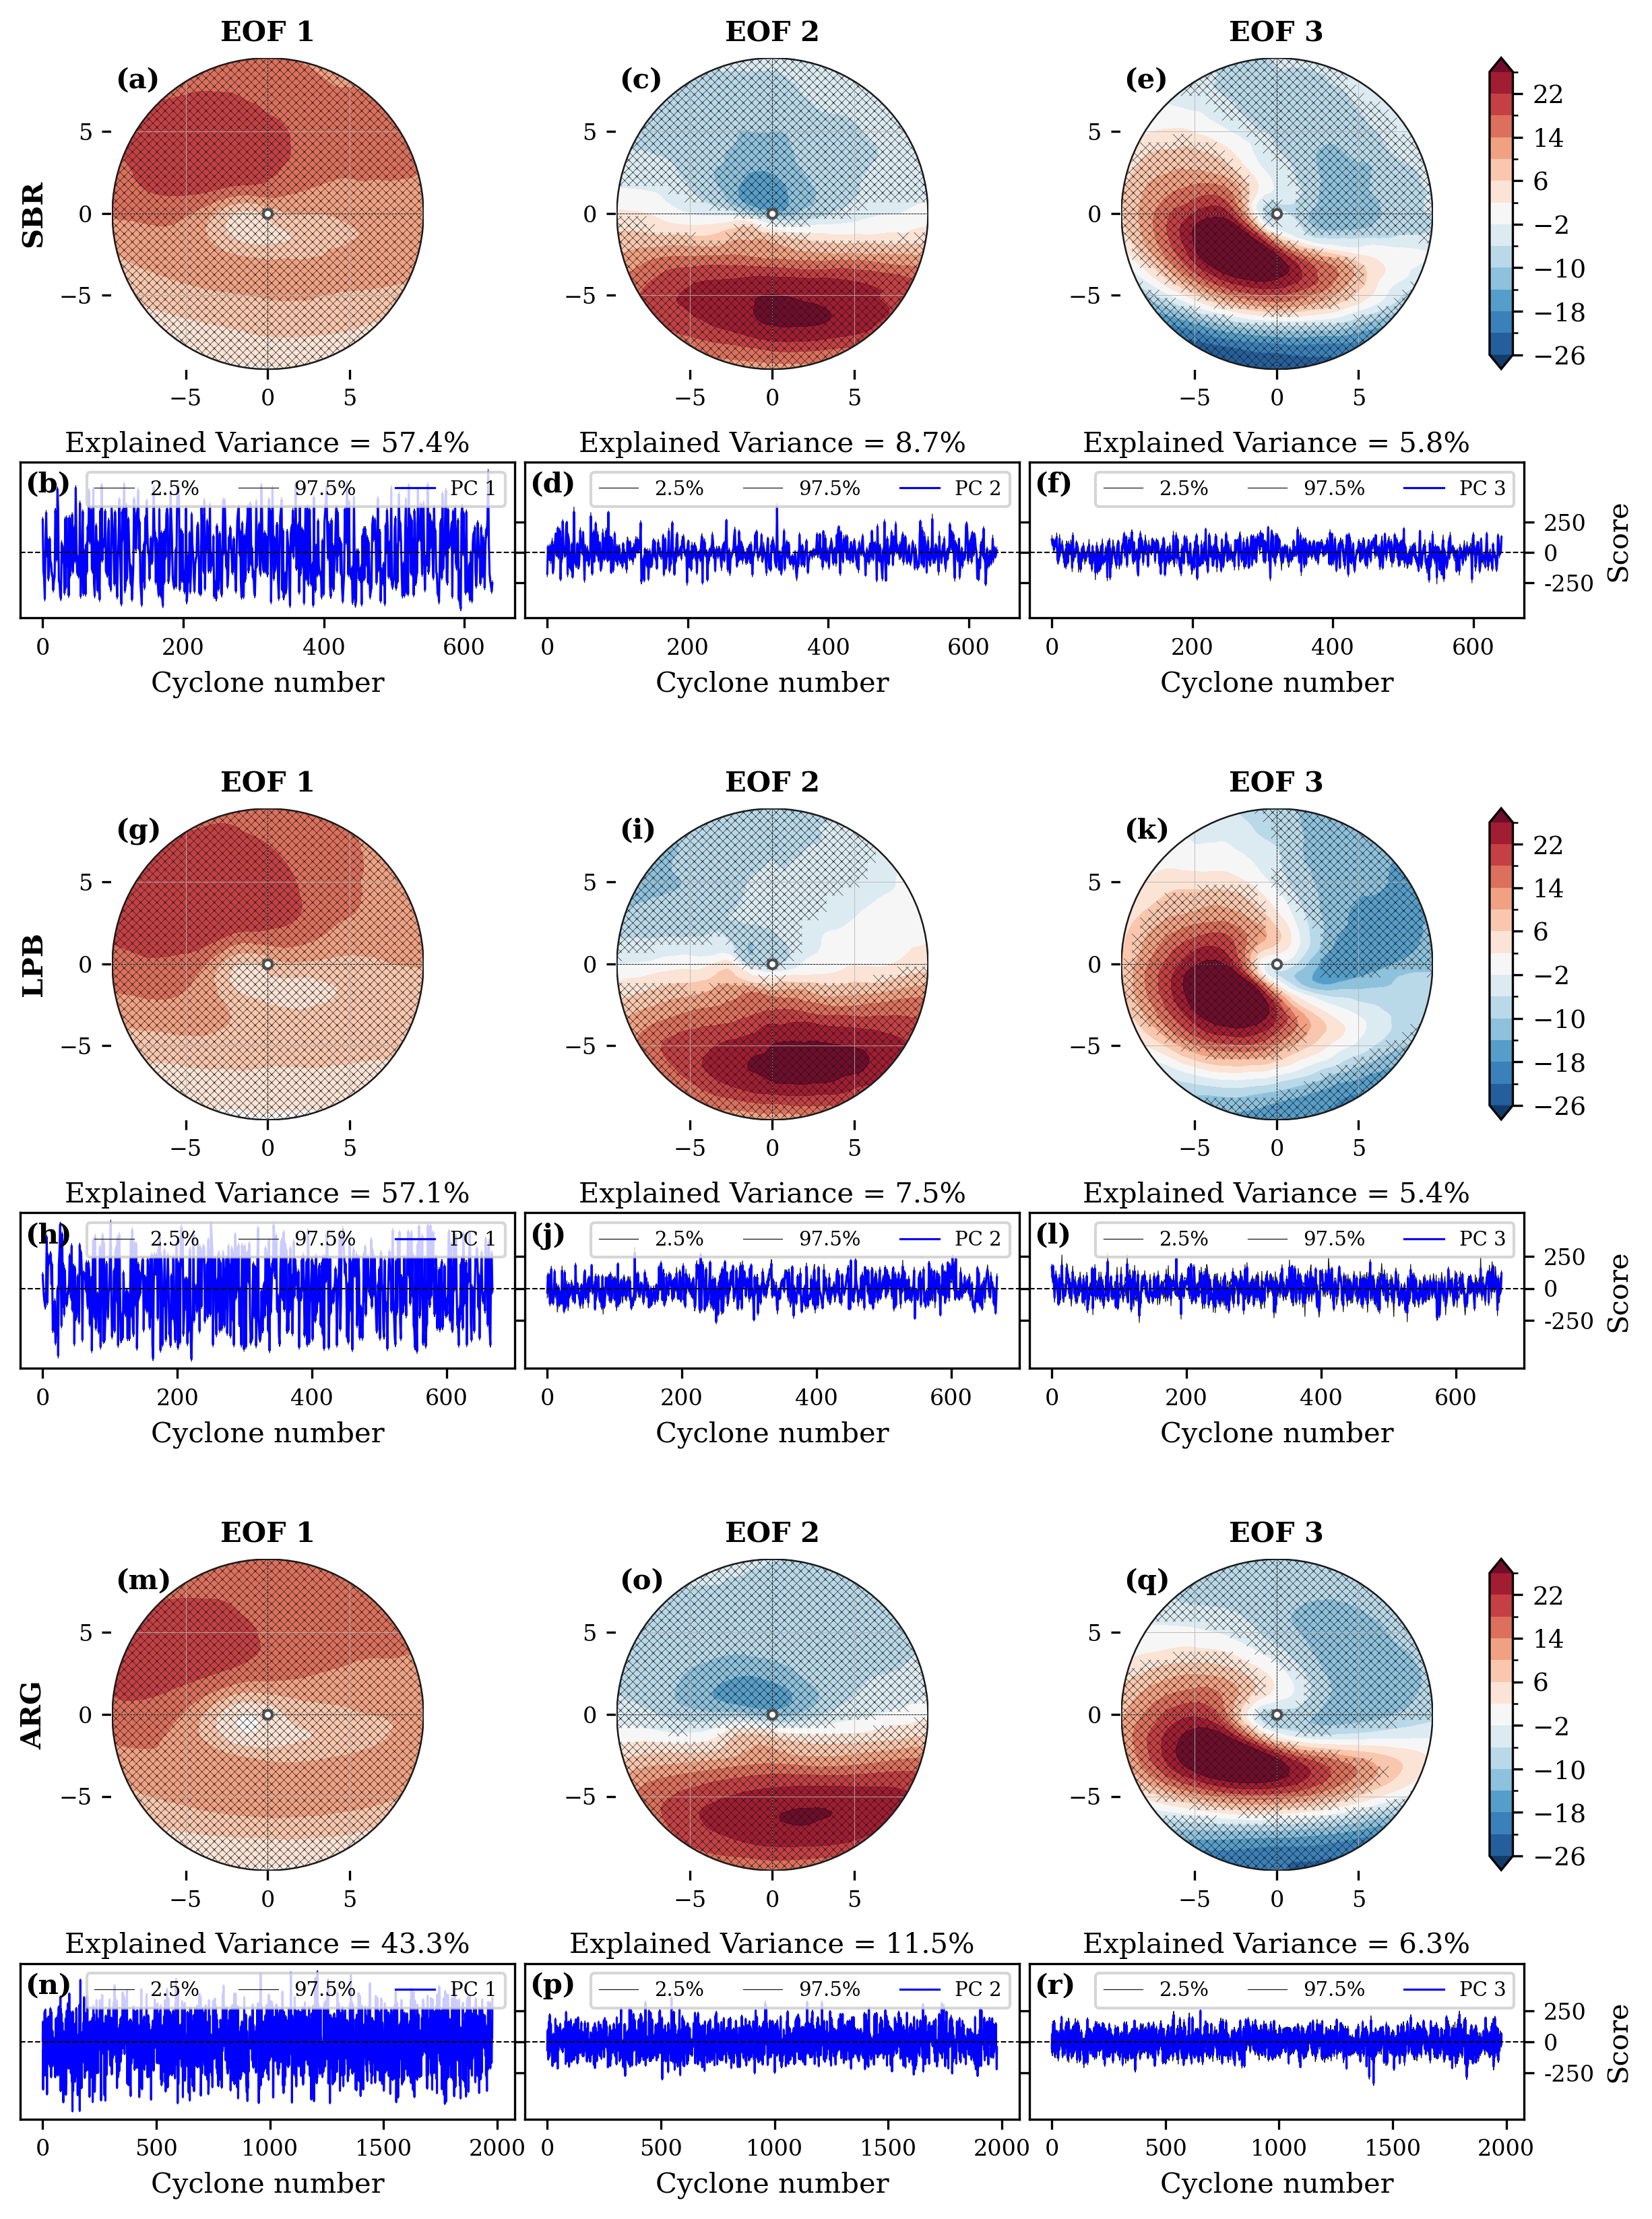
\includegraphics[width=\textwidth]{images/w10/xeof_global_wind10_mature.png}
\caption[Significancia espacial de los EOFs en fase de madurez --- Población Global]{Descomposición EOF del viento a 10~m para la Población Global en fase de madurez. Paneles (a, g, m): mapas de EOF1 para SBR, LPB y ARG respectivamente; (c, i, o): EOF2; (e, k, q): EOF3. El achurado indica significancia estadística al 95\% (test Bootstrap-t; Sección~\ref{subsec:bootstrap_significancia}). Paneles (b, h, n): series temporales de PC1; (d, j, p): PC2; (f, l, r): PC3. La línea gris delimita los percentiles 2.5 y 97.5 de la distribución bootstrap.}
\label{fig:xeof_madurez_global}
\end{figure}

\begin{figure}[htbp]
\centering
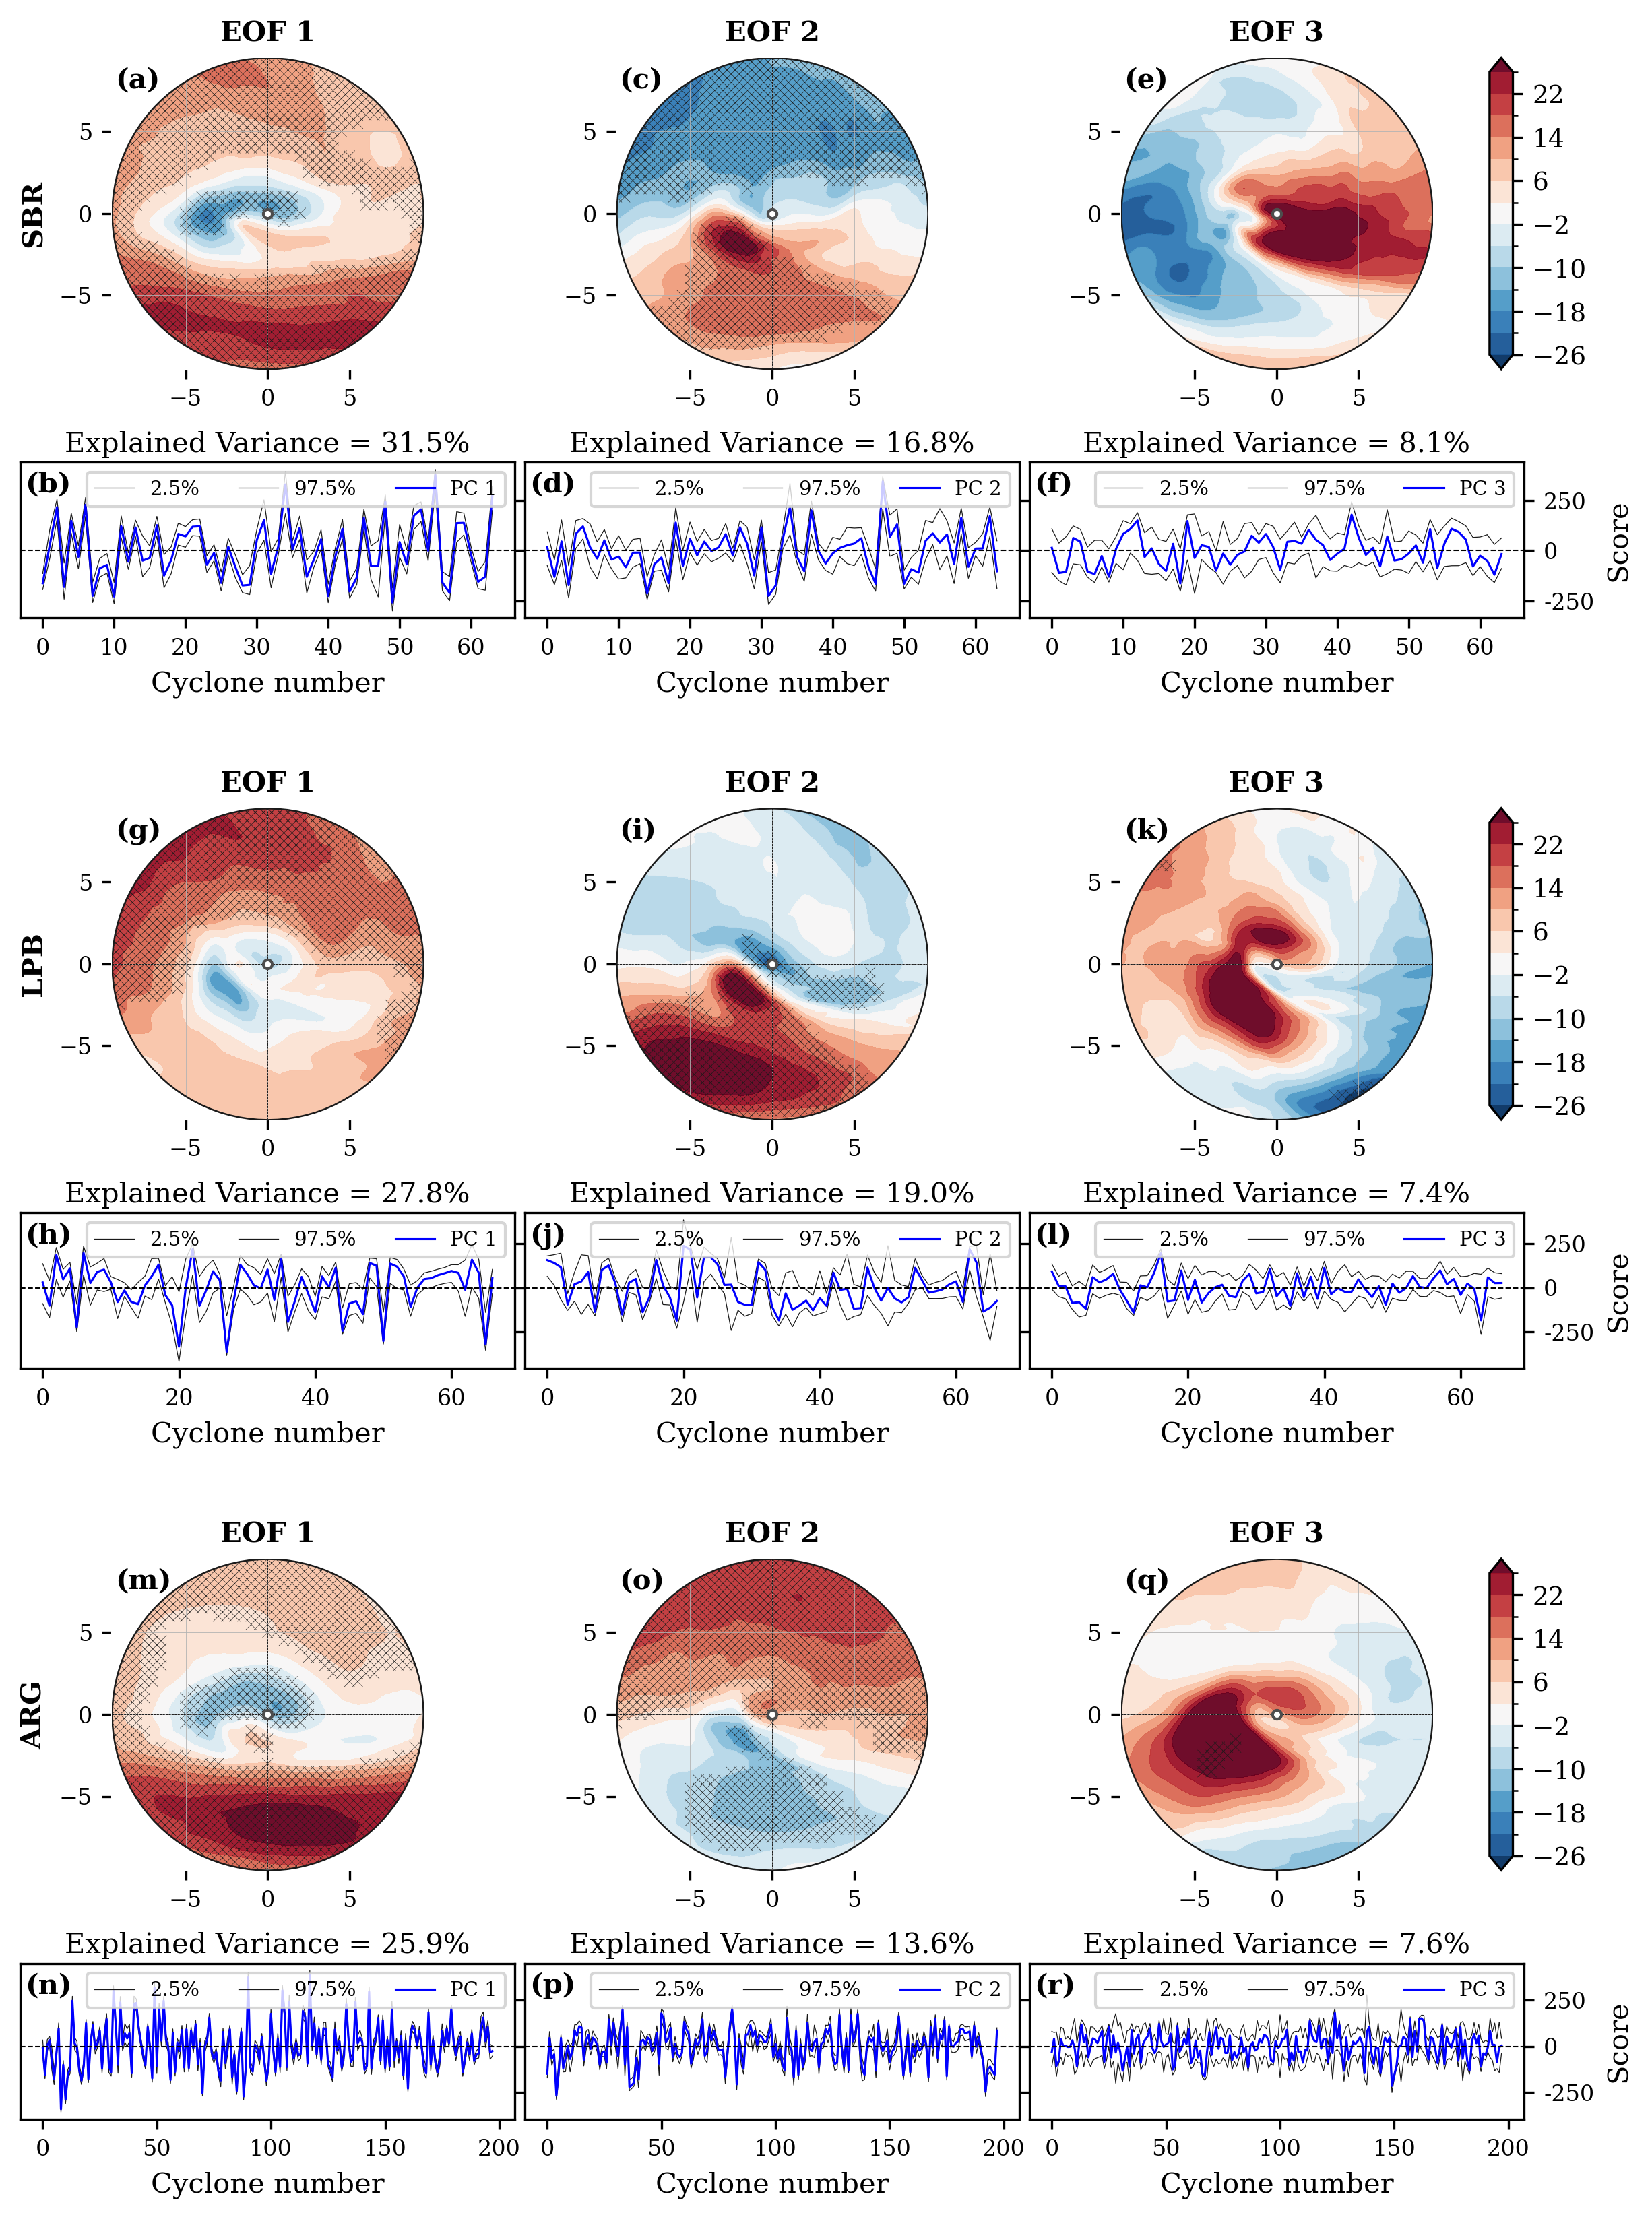
\includegraphics[width=\textwidth]{images/w10/xeof_p90_wind10_mature.png}
\caption[Significancia espacial de los EOFs en fase de madurez --- Subconjunto p90]{Descomposición EOF del viento a 10~m para el subconjunto intenso (p90) en fase de madurez. La disposición de paneles es idéntica a la Figura~\ref{fig:xeof_madurez_global}.}
\label{fig:xeof_madurez_p90}
\end{figure}

En la Población Global (Figura~\ref{fig:xeof_madurez_global}), EOF1 exhibe significancia que abarca el dominio total del sistema ciclónico en las tres regiones (paneles a, g, m para SBR, LPB y ARG). Esta respuesta puede asociarse al incremento de la conversión barotrópica de energía durante la madurez que \citet{coutodesouza2024thesis} documenta, es decir, el patrón constituye una característica física estable de los sistemas maduros. Consistente con la alta varianza explicada (43--57\%), las series de PC1 (paneles b, h, n) presentan amplitudes mayores que los modos secundarios; SBR y LPB muestran fluctuaciones comparables en PC1, mientras ARG exhibe dispersión ligeramente mayor e irregular.

Los modos EOF2 y EOF3 de la Población Global exhiben estructuras significativas confinadas a sectores específicos: EOF2 muestra la transición latitudinal respecto al centro (patrón positivo a negativo en las tres regiones), y EOF3 el gradiente zonal. EOF2 captura, por construcción, la varianza ortogonal al modo dominante \citep{hannachi2007empirical}; en este campo de viento, esa componente secundaria recuerda a fluctuaciones de circulación de mesoescala y asimetría secundaria. SBR y ARG presentan estructuras significativas de EOF2 más extendidas (paneles c y o) que LPB (panel i), donde no es significativa en el cuadrante noreste. Esta diferencia se refleja en las series temporales. Las PC2 de SBR (panel d) muestran episodios de alta amplitud más frecuentes que en LPB (panel j), indicando mayor variabilidad de mesoescala en SBR.

Las PC3 mantienen amplitudes atenuadas en las tres regiones (paneles f, l, r), consistente con su menor varianza explicada (5.4--6.3\%). Dado que en la Población Global la separación entre autovalores es pronunciada, los modos secundarios describen variabilidad residual de menor magnitud física. Sin embargo, ARG concentra mayor variabilidad explicada por EOF2 (11.5\%) que SBR (8.7\%) y LPB (7.5\%), sugiriendo que ARG experimenta procesos de mayor complejidad dinámica durante la madurez. En contraste, la estructura de EOF3 es notablemente similar entre regiones (5.4--6.3\%), indicando que los gradientes zonales de viento constituyen un mecanismo general de variabilidad residual en fase madura.

En el subconjunto p90 (Figura~\ref{fig:xeof_madurez_p90}), el patrón de significancia se transforma cualitativamente. EOF1 presenta una contracción variable entre regiones: en SBR (panel a) y ARG (panel m), la significancia se concentra en las áreas de anomalía positiva (sur y sureste, respectivamente), mientras sobre el núcleo negativo (nor-noroeste en SBR, noroeste en ARG) es más limitada, aunque no ausente. En LPB (panel g), la significancia permanece extensa en la región positiva del norte y noroeste, cubriendo parcialmente el noreste, excepto alrededor del centro, donde las anomalías negativas no son significativas. Esta reducción sugiere que EOF1 captura preferentemente una envolvente de mayor escala, sin llegar a representar de forma estadísticamente robusta algunas estructuras más localizadas de los ciclones intensos.

El contraste más relevante de p90 reside en EOF2 y EOF3. A diferencia de la Población Global, donde son residuales, en p90 estos modos (paneles c, i, o y e, k, q) presentan áreas de significancia que en varios casos superan en extensión a la del propio EOF1. Morfológicamente, EOF2 exhibe estructuras compactas e hiperlocalizadas alrededor del núcleo ciclónico en las tres regiones, en la zona donde suele ubicarse el chorro de la cinta transportadora fría (CCB). El chorro de bajo nivel que se forma en la cola del frente doblado (\textit{bent-back front}) responde al mismo mecanismo de intensificación por vorticidad potencial descrito para la CCB (Sección~\ref{sec:pdf_wind10}) \citep{schemm2014linkage}.

El comportamiento de las series temporales refuerza este diagnóstico. En la Población Global, PC2 y PC3 (paneles d, f para SBR; j, l para LPB; p, r para ARG) presentan amplitudes menores a los límites de PC1. En p90, las amplitudes de PC2 (paneles d, j, p) y PC3 (paneles f, l, r) son frecuentemente comparables a las de PC1 (paneles b, h, n). Los modos secundarios de p90 han dejado de ser ruido estadístico, consistente con el aplanamiento del espectro de autovalores ya discutido (Sección~\ref{sec:var_exp_wind10}).

La competencia energética entre PC1, PC2 y PC3 en p90 es la expresión estadística de la fragmentación dinámica del campo de viento (Sección~\ref{sec:var_exp_wind10}). La CCB, los frentes y las seclusiones térmicas compiten simultáneamente por la energía cinética del sistema, obligando a distribuir la varianza entre múltiples dimensiones ortogonales. En conjunto, estos resultados cuantifican la reducción de predictibilidad espacial asociada a la intensidad ciclónica. En la Población Global, el patrón dipolar débil estadísticamente robusto del EOF1 permite caracterizar la distribución del campo de viento mediante un único modo dominante. En p90, la señal de EOF1 se restringe a una envolvente de mayor escala, mientras la variabilidad más localizada, donde se concentran los vientos más extremos, queda capturada por EOF2 y EOF3; su significancia estadística en p90 confirma que esos patrones espaciales son reales y recurrentes, más allá del mecanismo puntual que se les atribuya.

\section{Componentes principales (PC1)}\label{subsec:res_dinamica_pc1}

La fragmentación de la varianza y la contracción de las áreas significativas en madurez (Sección~\ref{subsec:res_significancia_madurez}) tienen su contraparte en las Componentes Principales. Mientras en la Población Global PC1 domina la evolución del sistema, con amplitudes superiores y áreas significativas extensas, en los ciclones p90 la competencia entre múltiples modos ortogonales (Figura~\ref{fig:xeof_madurez_p90}) se traduce en propiedades estadísticas distintivas: aunque PC1 mantiene una correlación fuerte y consistente con la vorticidad en todas las fases, PC2 y PC3 dejan de ser ruido residual y capturan una fracción no despreciable de esa asociación con la intensidad.

\begin{table}[htbp]
\centering
\caption[Momentos estadísticos y correlación de PC1--PC3 del viento a 10 m - Población Global]
{Asimetría ($\gamma_1$) y curtosis ($\gamma_2$) de la PC1 del viento a 10 metros, y correlación de Spearman ($r$) entre PC1, PC2 y PC3 (con signo) y la vorticidad relativa a 850 hPa asociada a la fase (con signo, negativa en el Hemisferio Sur), para la Población Global. El signo de la correlación depende de la convención de signo de cada EOF (Sección~\ref{subsec:analisis_pc}); lo relevante es que el lado del patrón dominante en que cae cada ciclón está asociado a su intensidad. Los valores significativos ($p<0.05$) se muestran en negrita.}
\label{tab:stat_global_w10}
\begin{tabular*}{\textwidth}{@{\extracolsep{\fill}}llrrrrr}
\hline
\textbf{Región} & \textbf{Fase} & \textbf{Asimetría ($\gamma_1$)} & \textbf{Curtosis ($\gamma_2$)} & \textbf{PC1} & \textbf{PC2} & \textbf{PC3} \\
\hline
\textbf{SBR} & Incipiente       & 0.58  & -0.12 & \textbf{-0.57} & \textbf{0.20} & \textbf{-0.37} \\
             & Intensificación & 0.26  & -0.91 & \textbf{-0.80} & 0.02 & \textbf{-0.32} \\
             & Madurez         & 0.30  & -0.86 & \textbf{-0.89} & 0.04 & \textbf{-0.25} \\
             & Decaimiento     & 0.24  & -0.79 & \textbf{-0.83} & \textbf{0.12} & \textbf{0.13} \\
\hline
\textbf{LPB} & Incipiente       & 0.99  & 1.32  & \textbf{-0.35} & \textbf{0.14} & \textbf{0.16} \\
             & Intensificación & 0.17  & -1.03 & \textbf{-0.71} & \textbf{-0.18} & \textbf{-0.12} \\
             & Madurez         & -0.09 & -1.01 & \textbf{-0.87} & \textbf{-0.09} & \textbf{-0.19} \\
             & Decaimiento     & -0.11 & -0.77 & \textbf{-0.83} & \textbf{-0.11} & \textbf{-0.09} \\
\hline
\textbf{ARG} & Incipiente       & 0.31  & -0.13 & \textbf{-0.43} & \textbf{0.24} & \textbf{0.06} \\
             & Intensificación & -0.22 & -0.37 & \textbf{-0.67} & \textbf{0.11} & \textbf{0.05} \\
             & Madurez         & -0.12 & -0.43 & \textbf{-0.86} & \textbf{0.05} & \textbf{-0.26} \\
             & Decaimiento     & -0.06 & -0.30 & \textbf{-0.76} & -0.04 & \textbf{-0.28} \\
\hline
\end{tabular*}
\end{table}


\subsection{Población Global: modo dominante y su acoplamiento con la intensidad}\label{subsec:pc1_global_wind10}

La Tabla~\ref{tab:stat_global_w10} documenta las métricas estadísticas (asimetría, curtosis) y la correlación de Spearman entre PC1, PC2 y PC3 (con signo) y la vorticidad relativa a 850~hPa asociada a la fase (con signo), para la Población Global, calculadas según el procedimiento de la Sección~\ref{subsec:analisis_pc}.

La distribución de PC1 exhibe una progresiva normalización estructural. En las tres regiones, los valores de curtosis oscilan entre $-0.37$ y $-1.03$ durante intensificación y madurez, evidenciando distribuciones platicúrticas sin colas extremas dominantes. LPB muestra la mayor variabilidad inicial (asimetría $+0.99$, curtosis $+1.32$ en fase incipiente), mientras SBR y ARG presentan poblaciones más homogéneas desde etapas tempranas. El rasgo evolutivo más contundente emerge en el acoplamiento con la vorticidad. En todas las regiones, la correlación inicial de PC1, entre $-0.35$ (LPB) y $-0.57$ (SBR), se fortalece sistemáticamente hasta un máximo en madurez ($-0.890$ en SBR, $-0.868$ en LPB y $-0.860$ en ARG), cayendo levemente en decaimiento ($r < -0.75$). Esto indica que el lado del patrón dominante en que cae cada ciclón está sistemáticamente asociado a la intensidad del sistema, cada vez más a medida que el vórtice madura. PC2 alcanza significancia estadística en la mayoría de las combinaciones región-fase, con magnitudes moderadas ($|r| \leq 0.24$); PC3, en cambio, resulta significativo en las doce combinaciones región-fase y alcanza hasta $-0.37$ (SBR incipiente) y $-0.32$ (SBR intensificación), magnitudes menores a las de PC1 pero no despreciables. Esto matiza, ya en la Población Global, la idea de que PC2 y PC3 sean puro ruido residual, aunque su peso siga siendo consistentemente menor al de PC1 en esta población.

La progresiva simetrización de PC1 (asimetría tendiendo a cero) evidencia que, al intensificarse el vórtice, los campos de viento convergen hacia una configuración prototípica dominada por el primer modo de variabilidad. 
Para la mayoría de los ciclones, la distribución espacial del viento no es arbitraria, sino que se organiza en torno a un patrón coherente (EOF1); y en los ETCs de p90 se rompe dicha organización.
SBR exhibe acoplamiento desde etapas incipientes, mientras LPB requiere la fase de intensificación para alcanzarlo (pasando de $r = -0.35$ a $-0.71$), reflejando su carácter transicional donde la organización frontal emerge solo cuando el forzante baroclínico se establece con suficiente intensidad (Sección~\ref{subsec:tb_lpb}) --la misma fase en la que el PDFe ya mostraba a LPB alcanzando su núcleo de mayor densidad espacial (Sección~\ref{sec:kde_espacial_global}).

\begin{table}[htbp]
\centering
\caption[Momentos estadísticos y correlación de PC1--PC3 del viento a 10 m - Subconjunto p90]
{Asimetría ($\gamma_1$) y curtosis ($\gamma_2$) de la PC1 del viento a 10 metros, y correlación de Spearman ($r$) entre PC1, PC2 y PC3 (con signo) y la vorticidad relativa a 850 hPa asociada a la fase (con signo, negativa en el Hemisferio Sur), para el subconjunto extremo (p90). El signo de la correlación depende de la convención de signo de cada EOF (Sección~\ref{subsec:analisis_pc}); lo relevante es que el lado del patrón dominante en que cae cada ciclón está asociado a su intensidad. Los valores significativos ($p<0.05$) se muestran en negrita.}
\label{tab:stat_p90_w10}
\begin{tabular*}{\textwidth}{@{\extracolsep{\fill}}llrrrrr}
\hline
\textbf{Región} & \textbf{Fase} & \textbf{Asimetría ($\gamma_1$)} & \textbf{Curtosis ($\gamma_2$)} & \textbf{PC1} & \textbf{PC2} & \textbf{PC3} \\
\hline
\textbf{SBR} & Incipiente       & 0.16  & -0.56 & \textbf{-0.53} & 0.08 & \textbf{-0.58} \\
             & Intensificación & -0.25 & -0.65 & \textbf{-0.45} & \textbf{-0.27} & \textbf{0.58} \\
             & Madurez         & 0.36  & -0.55 & \textbf{-0.44} & 0.19 & -0.12 \\
             & Decaimiento     & 1.15  & 3.95  & \textbf{-0.66} & \textbf{-0.37} & 0.20 \\
\hline
\textbf{LPB} & Incipiente       & 0.77  & 0.42  & \textbf{-0.43} & 0.08 & -0.17 \\
             & Intensificación & -0.88 & 0.96  & \textbf{-0.45} & \textbf{-0.38} & \textbf{-0.49} \\
             & Madurez         & -0.93 & 0.60  & \textbf{-0.37} & 0.04 & -0.23 \\
             & Decaimiento     & -0.20 & -0.18 & \textbf{-0.54} & \textbf{-0.37} & \textbf{-0.56} \\
\hline
\textbf{ARG} & Incipiente       & 0.29  & -0.14 & \textbf{-0.43} & \textbf{0.21} & -0.09 \\
             & Intensificación & -0.38 & -0.19 & \textbf{-0.32} & \textbf{-0.15} & \textbf{-0.38} \\
             & Madurez         & 0.41  & 0.25  & \textbf{-0.26} & \textbf{-0.32} & \textbf{-0.33} \\
             & Decaimiento     & 0.51  & 1.66  & \textbf{-0.74} & -0.04 & \textbf{-0.20} \\
\hline
\end{tabular*}
\end{table}


\subsection{Subconjunto (p90): persistencia del acoplamiento con la vorticidad}\label{subsec:pc1_p90_wind10}

La Tabla~\ref{tab:stat_p90_w10} expone los parámetros estadísticos y las correlaciones (PC1--PC3, con signo) para el subconjunto extremo. A diferencia de la precipitación (Sección~\ref{subsec:pc1_p90_tp}), el acoplamiento entre PC1 y la vorticidad no colapsa en p90: se mantiene fuerte y significativo en las tres regiones y las cuatro fases, con valores entre $-0.26$ (ARG, madurez) y $-0.74$ (ARG, decaimiento). Esto indica que la organización del campo de viento en torno al modo dominante sigue ligada a la intensidad dinámica del sistema incluso en los eventos más extremos.

LPB exhibe leptocurtosis ($\gamma_2 = +0.96$) y asimetría negativa ($\gamma_1 = -0.88$) durante intensificación, reflejando una distribución de pico agudo con casos atípicos hacia valores bajos. SBR mantiene estabilidad durante el desarrollo pero exhibe un comportamiento marcadamente atípico en decaimiento, con leptocurtosis pronunciada ($\gamma_2 = +3.95$) y asimetría positiva ($+1.15$), evidenciando que los ciclones intensos no siguen un único camino estructural hacia la disipación.

El rasgo distintivo de p90 no es la pérdida de acoplamiento de PC1, sino la aparición de acoplamientos adicionales en PC2 y PC3 de mayor frecuencia y magnitud que en la Población Global (Sección~\ref{subsec:pc1_global_wind10}). En SBR intensificación, PC3 alcanza $r=0.58$ ($p<0.05$), más fuerte que el propio PC1 ($r=-0.45$); en ARG madurez, PC2 y PC3 también son significativos junto con PC1 ($r=-0.32$ y $-0.33$, respectivamente), mientras que en decaimiento es PC3 quien lo acompaña ($r=-0.20$), no PC2. Esto es consistente con la pérdida de dominancia de EOF1 documentada por el test Bootstrap-$t$ en la fase de madurez (Sección~\ref{subsec:res_significancia_madurez}): en p90, la energía cinética se reparte entre varios modos ortogonales asociados a estructuras mesoescalares (CCB, frente doblado), y esos modos secundarios también están ligados a la intensidad del vórtice, no solo el modo dominante.

Este hallazgo evidencia que, en los sistemas más intensos, el modo dominante (PC1) ya no concentra por sí solo la organización del campo de viento: aunque su acoplamiento con la vorticidad se mantiene, los modos secundarios capturan alteraciones internas de mesoescala que escapan de la linealidad sinóptica y que también están ligadas a la intensidad, por lo que parametrizar la respuesta del viento exclusivamente mediante el modo dominante resulta insuficiente. Esta limitación se inscribe en una discusión más amplia que plantea \citet{sinclair1997objective}, quien demuestra que la circulación, al integrar el tamaño y la rotación del sistema, constituye una medida más representativa de la intensidad real de un ciclón que la vorticidad local.

\section{Síntesis}\label{sec:sintesis_wind10}

El análisis del viento a 10~m muestra que el campo cinemático superficial a lo largo de las fases del ciclón no sigue una progresión lineal desde la población media hacia los ciclones más intensos.

\paragraph{Distribuciones de magnitud.}
La Población Global muestra distribuciones unimodales estrechas centradas en 12--15~m\,s$^{-1}$. En ciclones intensos (p90), el pico se desplaza a 20--23~m\,s$^{-1}$ (${\sim}$50\% superior) con colas de 30~m\,s$^{-1}$, consistente con registros previos para el Atlántico Sur. SBR y LPB alcanzan intensidades más extremas por advección cálida y convergencia de humedad, mientras que ARG exhibe distribuciones más anchas por dinámica baroclínica y efecto orográfico.

\paragraph{Localización espacial.}
En la Población Global los máximos se distribuyen difusamente con tendencia al cuadrante noroeste.
En p90, durante la madurez se hiperconcentran en el cuadrante noroeste a ${\sim}$3--4$^{\circ}$ del centro (densidades 23--27$\times10^{-4}$ en SBR), correspondiendo al chorro de la cinta transportadora fría (CCB) y a la fractura frontal.
En decaimiento, el núcleo asimétrico persiste en p90, mientras que en la Población Global se dispersa.

\paragraph{Estructura modal.}
En la Población Global, EOF1 domina ampliamente (43--57\%, máximo 57.4\% en SBR) con un dipolo norte--sur sinóptico.
En p90, la varianza se redistribuye entre múltiples modos competitivos (EOF1 $\leq$37.6\%).
El EOF1 de p90 en madurez presenta un núcleo negativo compacto rodeado de anomalías positivas, coherente con variabilidad de mesoescala; el núcleo hiperlocalizado de EOF2 coincide con la zona del chorro CCB, y en ARG con cambios en el tamaño de la seclusión cálida.

\paragraph{Acoplamiento dinámico.}
En la Población Global, la correlación entre PC1 y la vorticidad se fortalece hasta $r \approx -0.86$ a $-0.89$ en madurez.
En p90 este acoplamiento de PC1 no colapsa, se mantiene fuerte en las tres regiones y las cuatro fases (entre $-0.26$ en ARG-madurez y $-0.74$ en ARG-decaimiento), a diferencia de lo que ocurre con la precipitación (Capítulo~\ref{cap:resultados_tp}).
Lo distintivo de p90 es la aparición de acoplamientos adicionales en PC2 y PC3 de mayor frecuencia y magnitud (hasta $r=0.58$ en SBR-intensificación, superando al propio PC1) que en la Población Global, con leptocurtosis en LPB ($\gamma_2 = +0.96$) y leptocurtosis pronunciada en SBR en decaimiento ($\gamma_2 = +3.95$).

En consecuencia, el modo dominante (PC1) por sí solo no basta para describir completamente la organización del viento en los sistemas más intensos: aunque su acoplamiento con la vorticidad se mantiene, los vientos máximos de p90 también responden a procesos de mesoescala (seclusiones térmicas, CCB, descargas descendentes sobre la superficie frontal fría \citep{hyeok2024extrem}) capturados por los modos secundarios, exigiendo diagnósticos adicionales (estabilidad estática, humedad) durante la madurez.
SBR y LPB desarrollan núcleos de viento más intensos y coherentes por flujos de calor latente y orografía, mientras que ARG presenta mayor heterogeneidad estructural (Sección~\ref{sec:tb_regiones}).

\paragraph{Alcance e implicaciones.}
Estos resultados sugieren que, aunque la vorticidad relativa está sistemáticamente asociada al modo dominante de organización del viento incluso en los sistemas más intensos, un único modo no basta para anticipar completamente la severidad y ubicación del viento superficial en la fase más peligrosa: los modos secundarios, ligados a procesos de mesoescala, aportan información adicional que motiva incorporar diagnósticos complementarios (estabilidad, humedad, geometría frontal) en esquemas de alerta para el Atlántico Sur. Conviene, sin embargo, interpretar estas cifras con cautela, ya que el acoplamiento aquí reportado depende de la vorticidad asociada a la fase como métrica puntual de intensidad, y podría diferir si se emplea una medida integrada de circulación \citep{sinclair1997objective}. Asimismo, aunque \citet{gray2024global} confirma que el mecanismo de \textit{sting jet} opera en el Hemisferio Sur en su conjunto (Sección~\ref{sec:kde_espacial_p90}), su climatología no desagrega el Atlántico Sur de las demás cuencas del hemisferio, de modo que la extensión de este mecanismo a los ciclones aquí estudiados sigue apoyada más en la inversión especular de la circulación que en evidencia regional directa.

Esta base, que vincula la intensidad (p90) con una distribución espacial específica del viento máximo, constituye el punto de partida para evaluar la relación con la precipitación (Capítulo~\ref{cap:resultados_tp}), dado que el acoplamiento intensidad--precipitación está fuertemente condicionado por la organización del sistema \citep{sinclair2023relationship}.
La caracterización integrada de ambos campos mediante MEOF (Sección~\ref{sec:tb_compound_def}) permitirá evaluar si su organización espacial es coherente o está desacoplada según la fase evolutiva y la región de génesis.
